\documentclass[11pt]{article}
\usepackage[margin=1in]{geometry}
\usepackage{amsfonts, amsmath, amssymb}
\usepackage[none]{hyphenat}
\usepackage{fancyhdr}
\usepackage{graphicx}
\usepackage{float}
\usepackage[nottoc, notlot, notlof]{tocbibind}
\usepackage{apacite}
\usepackage[bottom]{footmisc}
\usepackage[italian]{babel}

\pagestyle{fancy}
\fancyhead{}
\fancyfoot{}
\fancyhead[L]{\slshape \MakeUppercase{Network Alignment}}
\fancyhead[R]{\slshape Luca Masiero, Stefano Ivancich}
\fancyfoot[C]{\thepage}
%\renewcommand{\headrulewidth}{0pt}
\renewcommand{\footrulewidth}{0pt}

%\parindent 0ex per l'indendazione
%\setlength{\parindent}{4em}
%\setlength{\parskip}{1em}
%\renewcommand{\baselinestretch}{1.5}
\begin{document}

\begin{titlepage}
\begin{center}
\vspace*{1cm}
\Large{\textbf{Università degli Studi di Padova}}\\
\Large{\textbf{Corso di Laurea Magistrale in Ingegneria Informatica}}\\
\begin{center}

\includegraphics[scale=0.2]{uni}
\end{center}
%\vfill
\line(1,0){470}\\[1mm]
\Huge{\textbf{\begin{huge}Progetto di \textit{Algoritmi per la Bioinformatica}\end{huge}}}\\[3mm]
\Huge{\textbf{Network Alignment}}\\[1mm]
\Large{\textbf{- PPI: Protein-Protein Interaction -}}\\[1mm]
\line(1,0){470}\\
\begin{flushright}
\textbf{Studenti}: \textit{Luca Masiero}\\\textit{Stefano Ivancich}
\end{flushright}

\begin{flushleft}
\textbf{Supervisor}: \textit{Prof. Matteo Comin}\\
\end{flushleft}
\vfill
\textbf{Anno Accademico 2019-2020}
 \\
18 Giugno 2020
\end{center}
\end{titlepage}
\setcounter{page}{1}
\newpage
%\begin{titlepage}
%\begin{center}
%\vspace*{1cm}
%\vfill
%\begin{flushright}
%\small{\textit{L'unica maniera per scoprire i limiti del possibile è avventurarsi poco al di là di essi nell'impossibile.}}\\
%\small{Arthur C. Clarke}\\
%\end{flushright}
%\vfill
%\end{center}
%\end{titlepage}
\tableofcontents %compila due volte per l'indice corretto!
\thispagestyle{empty}
\clearpage

\newpage
\section{Introduzione: \textit{Network Alignment} e \textit{PPIN}}
L'obiettivo del \textit{\textbf{Network Alignment}} (traducibile con \textit{allineamento delle reti}) consiste nel trovare somiglianze tra la struttura e/o la topologia di due o più reti. 

Nel contesto biologico, confrontare le reti di diversi organismi (rappresentate tramite \textit{grafi}) è, attualmente, uno dei problemi più importanti ed interessanti della Biologia. Gli allineamenti di reti biologiche possono infatti risultare molto utili perché, avendo molte informazioni su alcuni nodi di una determinata rete $G_1$ e quasi nulla su nodi topologicamente simili in un'altra $G_2$, la conoscenza specialistica di uno di quei nodi può dirci qualcosa di nuovo sul corrispettivo. Gli allineamenti delle reti possono anche essere utilizzati per misurare la somiglianza globale tra reti complete di specie diverse. 

Le \textit{\textbf{Protein-Protein Interaction Networks}} (\textbf{PPIN}, \textit{reti di interazione proteina-proteina}) sono strumenti validi per comprendere le funzioni delle cellule, le malattie umane e il design e riposizionamento dei farmaci\footnote{Il \textit{drug-repositioning} è l’insieme delle analisi volte a stabilire se un farmaco già noto possa essere utilizzato per il trattamento di sintomatologie diverse da quelle descritte in etichetta.}, nonché per ottenere una descrizione completa degli \textit{interattomi}\footnote{Si veda la \textit{\textbf{Sottosezione 2.1.}}} affinché sia possibile capire, tramite la loro analisi comparativa, più profondamente i processi biologici.

\begin{center}
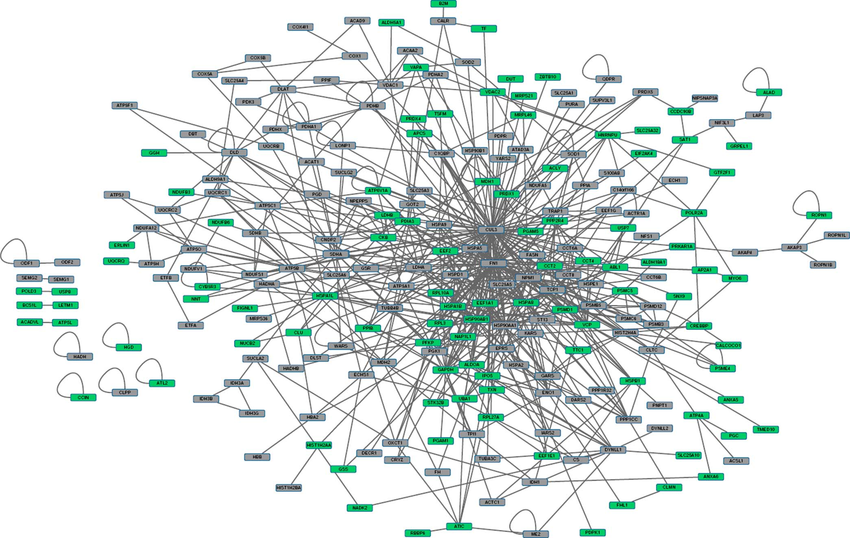
\includegraphics[scale=0.46]{woo}

\begin{small}\textit{\textbf{Figura 1.1}: Un esempio di PPIN.}\end{small}
\end{center}

Interpretare una PPI è un compito particolarmente impegnativo a causa della complessità della rete. Negli anni, sono stati proposti diversi algoritmi per l'interpretazione automatica delle PPI, in un primo momento considerando esclusivamente la \textit{topologia della rete}\footnote{La topologia di rete è il modello (grafo) finalizzato a rappresentare le relazioni di connettività, fisica o logica, tra gli elementi costituenti la rete stessa (i \textit{nodi}).}, e successivamente integrando i termini dell'\textit{Ontologia Genica}\footnote{Nato nel 1988, \textit{Gene Ontology} è un progetto bioinformatico atto a unificare la descrizione delle caratteristiche dei prodotti dei geni in tutte le specie. In particolare, il progetto si propone di: 
\begin{enumerate}
\setlength{\itemsep}{1pt}
  \setlength{\parskip}{0pt}
  \setlength{\parsep}{0pt}
\item Mantenere e sviluppare un vocabolario controllato atto a descrivere i geni e i prodotti genici per ogni organismo vivente;
\item Annotare i geni e i prodotti genici, e diffondere tali dati;
\item Fornire strumenti per un facile accesso ai dati forniti dal progetto.
\end{enumerate} 
} (GO) come attributi di somiglianza dei nodi. 



Negli ultimi anni, la crescente quantità e qualità dei dati "-omici"\footnote{Quando si parla di “scienze omiche” si intendono quelle discipline che hanno per oggetto di studio l’insieme di geni (genomica), dei trascritti (trascrittomica), delle proteine (proteomica) e dei metaboliti (metabolomica) che vengono espressi da una cellula, diversamente da quanto fanno le scienze biologiche tradizionali che invece si occupano di studiare i processi biologici singolarmente. Si tratta, dunque, di guardare cellule e tessuti da una prospettiva diversa, prospettiva che probabilmente meglio si addice a descrivere dei sistemi come quelli biologici caratterizzati da un elevato grado di complessità.} ha portato all'assemblaggio di reti biologiche, il cui obiettivo finale è quello di svelare i processi cellulari sottostanti. In questo scenario, le PPI sono tra le reti più importanti ed ampiamente studiate. Nelle reti PPI, un sistema biologico è descritto in termini di \textit{\textbf{proteine}}\footnote{Le proteine sono macromolecole biologiche costituite da catene di amminoacidi legati uno all'altro da un legame peptidico (ovvero un legame tra il gruppo amminico di un amminoacido e il gruppo carbossilico dell'altro amminoacido, creato attraverso una reazione di condensazione con perdita di una molecola d'acqua). Le proteine svolgono una vasta gamma di funzioni all'interno degli organismi viventi, tra cui la catalisi delle reazioni metaboliche, funzione di sintesi (come la replicazione del DNA), la risposta agli stimoli e il trasporto di molecole da un luogo ad un altro. Le proteine differiscono l'una dall'altra soprattutto nella loro sequenza di amminoacidi, la quale è dettata dalla sequenza nucleotidica conservata nei geni e che di solito si traduce in un ripiegamento proteico e in una struttura tridimensionale specifica che determina la sua attività.}, 
che costituiscono i \textit{nodi} del grafo, e le loro relazioni (interazioni fisico/funzionali), rappresentate dagli \textit{archi} del grafo.\\

Date le grandi dimensioni (tipicamente vengono coinvolte migliaia di elementi), le reti PPI sono analizzate tramite l'identificazione di \textit{sottoreti}, o \textit{moduli}, che mostrano specifiche caratteristiche topologiche e/o funzionali.

L'espressione \textbf{modulo topologico} si riferisce ad un \textit{gruppo di nodi che hanno molte più connessioni con i nodi del gruppo piuttosto che con quelli esterni}. 

L'espressione \textbf{modulo funzionale} si riferisce ad un \textit{gruppo di nodi che condividono una funzione biologica}. 

Si noti che un gruppo di nodi che rappresenta un modulo può avere sia proprietà topologiche che funzionali. Idealmente, i moduli topologici e funzionali coinciderebbero; in pratica, essi costituiscono due entità diverse, anche se tipicamente si sovrappongono in larga misura. Di conseguenza, sia la topologia della rete che le informazioni funzionali contribuiscono alla comprensione complessiva dei meccanismi biologici delle reti PPI.\\

Nella prossime sezioni presenteremo gli argomenti necessari per comprendere il funzionamento dei metodi attualmente più efficienti per l'analisi delle PPIN.

\newpage
\section{\textit{Protein-Protein Interaction Networks}}
Le \textit{\textbf{interazioni proteina-proteina}} (PPI) sono essenziali per quasi tutti i processi che avvengono all'interno di una cellula; comprendere a pieno queste interazioni è a sua volta fondamentale per studiare la fisiologia cellulare in condizioni normali o di malattia, o per sviluppare nuovi farmaci (dato che possono influenzare le PPI stesse). Le PPIN sono rappresentazioni matematiche dei contatti fisici tra le proteine all'interno della cellula. Questi contatti:
\begin{itemize}
\setlength{\itemsep}{1pt}
  \setlength{\parskip}{0pt}
  \setlength{\parsep}{0pt}
\item sono specifici;
\item si verificano tra le regioni di legame (\textit{binding regions}) nelle proteine;
\item hanno un particolare significato biologico (cioè svolgono una funzione specifica).
\end{itemize}
Le informazioni riguardanti le PPI possono rappresentare sia le interazioni transitorie che quelle stabili, in particolare:
\begin{itemize}
\setlength{\itemsep}{1pt}
  \setlength{\parskip}{0pt}
  \setlength{\parsep}{0pt}
\item Le interazioni \textit{stabili} si formano in complessi proteici (e.g. ribosoma\footnote{I ribosomi sono complessi macromolecolari, immersi nel citoplasma o ancorati al reticolo endoplasmatico ruvido o contenuti in altri organuli, responsabili della sintesi proteica. La loro funzione è quella di leggere le informazioni contenute nella catena di RNA messaggero.}, emoglobina\footnote{L'emoglobina è una proteina globulare mediante la quale si compie il trasporto dell'ossigeno dai polmoni ai tessuti e dell'anidride carbonica dai tessuti ai polmoni.}).
\item Le interazioni \textit{transitorie} sono brevi interazioni che modificano o trasportano una proteina, portando ad ulteriori cambiamenti; costituiscono la parte più dinamica dell'\textbf{interattoma}, di cui parleremo fra un attimo.
\end{itemize}

La conoscenza delle PPI può essere utilizzata per assegnare ruoli putativi\footnote{Presunto, apparente.} alle proteine non caratterizzate o caratterizzare le relazioni tra le proteine che formano complessi multimolecolari.

\subsection{L'interattoma}
L'\textbf{\textit{interattoma}}, rappresentato tramite grafo, è \textit{l'insieme complessivo delle interazioni molecolari in una particolare cellula} e costituisce la totalità delle PPI che si verificano all'interno della stessa, ma anche in un organismo o in un contesto biologico specifico. Lo sviluppo di tecniche di screening PPI su larga scala ha portato ad un'esplosione nella quantità di dati disponibili e la costruzione di interattomi sempre più complessi e completi (si veda la \textit{\textbf{Figura 2.1}}).

\begin{center}
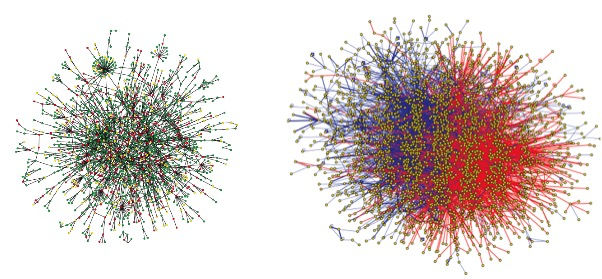
\includegraphics[scale=0.6]{interact}

\begin{small}\textit{\textbf{Figura 2.1}: Interattoma del lievito (sinistra) ed interattoma umano (destra)}.\end{small}
\end{center}

A questo punto, tuttavia, è necessario sottolineare i limiti dei dati PPI disponibili. La nostra attuale conoscenza dell'interattoma è purtroppo incompleta e rumorosa (\textit{noisy}). I metodi di rilevamento delle PPI hanno dei limiti per quanto riguarda il numero di interazioni veramente fisiologiche che possono essere rilevate e tutti i metodi per ora realizzati ed implementati individuano sia falsi positivi che negativi.

\section{PPIN: proprietà fondamentali}
In questa sezione diamo uno sguardo generale ad alcune delle proprietà più importanti delle PPIN.

\subsection{\textit{Effetto del piccolo mondo}}
Le \textit{reti di interazione proteina-proteina} sono soggette all'\textit{effetto del piccolo mondo}\footnote{L'\textit{effetto del mondo piccolo} è una teoria che sostiene che tutte le reti complesse presenti in natura sono tali che due nodi qualsiasi possono essere collegati da un percorso costituito da un numero relativamente piccolo di collegamenti.}, ciò significa che intercorre una grande connettività tra le proteine (\textit{\textbf{Figura 3.1}}). In altre parole, si può dire che il \textit{diametro} della rete (= numero massimo di "passi" che separano due nodi qualsiasi) è piccolo, non importa quanto grande sia la rete\footnote{Questo, di solito, significa che due nodi sono separati da meno di sei passi (che riflettono l'ormai ampiamente diffusa teoria dei \textit{sei gradi di separazione} usata nelle scienze sociali).}.

\begin{center}
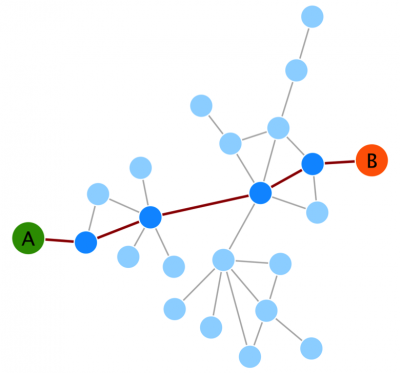
\includegraphics[scale=0.4]{grafo}

\begin{small}\textit{\textbf{Figura 3.1}: Effetto del piccolo mondo}.\end{small}
\end{center}

Questo livello di connettività ha importanti conseguenze biologiche, poiché consente un flusso efficiente e rapido dei segnali all'interno della rete stessa. 

A questo punto sorge spontanea una domanda: \textit{se la rete è così strettamente connessa, perché le perturbazioni in un singolo gene o in una singola proteina non hanno conseguenze drammatiche per la rete?} I sistemi biologici sono estremamente robusti e possono far fronte a una quantità relativamente elevata di perturbazioni in singoli/e geni/proteine. Per spiegare come ciò possa accadere, dobbiamo considerare un'altra proprietà fondamentale delle PPIN, che vedremo nella prossima sottosezione.

\subsection{\textit{Scale-free networks}}
Le PPIN sono \textit{\textbf{scale-free networks}}. La maggior parte dei nodi (che corrispondono alle proteine) nelle \textit{scale-free networks} hanno solo poche connessioni con altri nodi, mentre altri (denominati \textit{hub}) sono collegati a molti altri nodi della rete stessa (\textit{\textbf{Figura 3.2}}).

\begin{center}
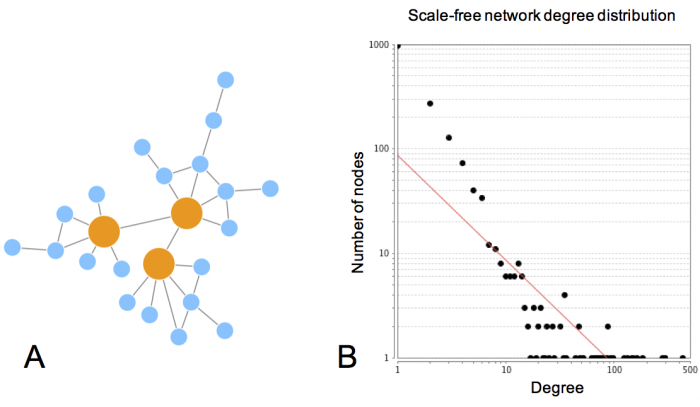
\includegraphics[scale=0.53]{graffo}

\begin{small}\textit{\textbf{Figura 3.2}: Il numero di connessioni di ogni nodo è chiamato \textbf{grado}. Se rappresentiamo la distribuzione del grado di una \textit{scale-free network} in scala logaritmica, possiamo notare come si adatti ad una linea, avendo un piccolo numero di nodi con un alto grado (gli hub) e un grande numero di nodi con un basso grado}.\end{small}
\end{center}

Le \textit{scale-free networks} possono essere costruite seguendo il modello di collegamento preferenziale, noto anche come il principio "\textit{rich get richer}" (tali reti possono essere create aggiungendo archi che sono preferibilmente collegati a nodi con un grado più elevato).

La natura \textit{scale-free} delle reti di interazione proteina-proteina conferisce loro una serie di importanti caratteristiche:
\begin{enumerate}
\setlength{\itemsep}{1pt}
  \setlength{\parskip}{0pt}
  \setlength{\parsep}{0pt}
\item \textbf{Stabilità}
\begin{itemize}
\setlength{\itemsep}{1pt}
  \setlength{\parskip}{0pt}
  \setlength{\parsep}{0pt}
\item Se i guasti si verificano in modo casuale e la maggioranza delle proteine costituisce un grado di connettività basso, la probabilità che un \textit{hub} venga colpito è minima.
\item Se si verifica un \textit{hub-failure}, la rete generalmente non perde la sua connettività grazie ai restanti \textit{hub}.
\end{itemize}

\item \textbf{Invarianza ai cambiamenti di scala}
\begin{itemize}
\item Non importa quanti nodi o archi abbia la rete, le sue proprietà rimangono stabili.
\item La presenza di nodi è ciò che consente l'\textit{effetto piccolo mondo} indipendentemente dalle dimensioni della rete.
\end{itemize}

\item \textbf{Vulnerabilità agli attacchi mirati}
\begin{itemize}
\item Se si perdono alcuni \textit{hub} principali, la rete si trasforma in un insieme di grafi isolati.
\end{itemize}
\end{enumerate}

\subsection{Transitività}
Un'altra caratteristica cruciale delle PPIN è la loro modularità\footnote{Caratteristica di un sistema che si compone di unità distinte (\textit{moduli}), ognuna delle quali assolve un compito specifico ed è capace di interagire con le altre.}. La \textit{\textbf{transitività}} o \textit{coefficiente di clustering} di una rete misura la tendenza dei nodi a raggrupparsi. Un'alta transitività significa che la rete contiene "comunità" o gruppi di nodi che sono densamente connessi (seguendo un'analogia delle scienze sociali, "gli amici dei miei amici sono miei amici"). Nelle reti biologiche, trovare queste comunità è molto importante perché possono aiutare ad individuare  \textbf{complessi proteici} (a titolo di esempio, si veda la \textit{\textbf{Figura 3.3}}).

\begin{center}
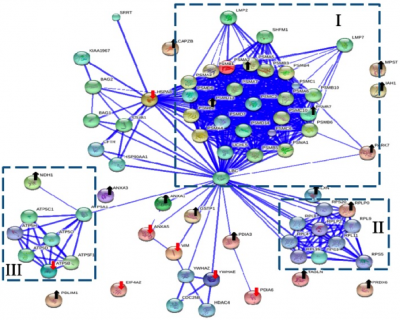
\includegraphics[scale=0.65]{grafffo}

\begin{small}\textit{\textbf{Figura 3.3}: Cluster topologici che riflettono la funzione biologica. I cluster sono evidenziati all'interno di quadrati a linee tratteggiate}.\end{small}
\end{center}

I \textit{complessi proteici} possono essere considerati un tipo di \textit{\textbf{modulo}} (un'unità funzionale ed intercambiabile) in cui le proteine interagiscono in modo stabile, mantenendo una configurazione più o meno costante sia nel tempo che nello spazio.

Lo studio dei moduli è utile anche per definire le \textit{interazioni intermodulari} tra le proteine.

\newpage
\section{PPIN: sorgenti di dati, affidabilità e confidenza}
Il primo passo per eseguire l'analisi delle PPIN è, naturalmente, la costruzione di una rete. Ci sono diverse fonti di dati PPI che possono essere utilizzate ed è importante essere consapevoli dei loro vantaggi e svantaggi.

Essenzialmente, è possibile ottenere dati PPI da:
\begin{enumerate}
\setlength{\itemsep}{1pt}
  \setlength{\parskip}{0pt}
  \setlength{\parsep}{0pt}
\item \textbf{Il proprio lavoro sperimentale}, dove si può scegliere come i dati verranno rappresentati e memorizzati.
\item \textbf{Un database primario di PPI}. Questi database estraggono le PPI dalle prove sperimentali riportate in letteratura utilizzando un processo di cura manuale. Costituiscono i principali fornitori di dati PPI.
\item \textbf{Un database di metadati\footnote{Informazione che descrive un insieme di dati.} o un database predittivo}. Queste risorse riuniscono le informazioni fornite da diversi database primari e forniscono all'utente una rappresentazione unificata dei dati. 
I database predittivi vanno oltre e utilizzano i set di dati prodotti in modo sperimentale per prevedere, dal punto di vista puramente computazionale, le interazioni in aree inesplorate dell'interattoma. Questi dataset, tuttavia, sono in genere più "rumorosi" di quelli provenienti da altre fonti.
\end{enumerate}

Spesso sarà necessario integrare dati PPI provenienti da più fonti, poiché nessun database ha una rappresentazione completa di tutte le informazioni necessarie. Da questo fatto derivano alcune sfide interessanti, poiché diversi database utilizzano  identificatori diversi e contengono diversi tipi di dati.\\

A questo punto sorge una preoccupazione che ha a che fare con l'analisi della rete: \textit{ci si può "fidare" del fatto che la rete di interazione rappresenti una "reale" interazione biologica?} Dato il rumore (\textit{noise}) insito nelle informazioni dell'interattoma, è importante essere rigorosi e attenti quando si valutano i dati delle \textit{interazioni proteina-proteina} che si utilizzano (potremmo infatti trovarci di fronte a rindondanze ed incoerenze). È molto importante tener conto del fatto che l'interattoma potrebbe essere incompleto o frammentario, per questo motivo esistono modi diversi per accertare l'affidabilità dei dati che si stanno considerando. Alcune strategie si avvalgono dei seguenti metodi:
\begin{enumerate}
\setlength{\itemsep}{1pt}
  \setlength{\parskip}{0pt}
  \setlength{\parsep}{0pt}
\item \textbf{Informazioni biologiche contestuali} riguardanti le proteine e/o le molecole che sono coinvolte nell'interazione.
\item \textbf{Contare quante volte una data interazione è stata riportata in letteratura}. Questo è un approccio molto popolare e semplice; esistono varianti più elaborate di questa strategia, come il metodo MIscore\footnote{Per una descrizione completa e rigorosa di questo metodo rimandiamo alla lettura del seguente paper (non inserito nella \textbf{Bibliografia}): Villaveces, J.M., et al., Merging and scoring molecular interactions utilising existing community standards: tools, use-cases and a case study. Database (Oxford), 2015. 2015. }.
\item \textbf{Metodi aggregati} che utilizzano una serie di strategie diverse e le integrano in un unico punteggio, come INTscore\footnote{A titolo informativo, il paper (non inserito nella \textbf{Bibliografia}) riguardante INTscore è il seguente: Kamburov, A., Stelzl, U., and Herwig, R. IntScore: a web tool for confidence scoring of biological interactions. Nucleic Acids Res, 2012. 40(Web Server issue): p. W140-6.}.
\end{enumerate}

\section{PPIN: analisi topologica}
L'analisi delle caratteristiche topologiche di una rete è un modo utile per identificare i partecipanti e le sottostrutture rilevanti che possono avere un significato dal punto di vista biologico. Ci sono molte strategie diverse che possono essere usate per fare ciò (si veda la \textit{\textbf{Figura 5.1}}); in questa sezione ci concentreremo sull'analisi della centralità (\textit{centrality analysis}) e sul clustering topologico (\textit{topological clustering}).

\begin{center}
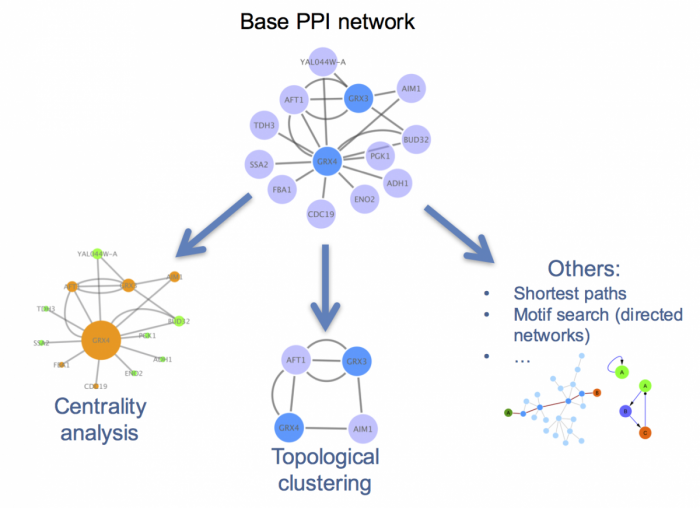
\includegraphics[scale=0.35]{ppin}

\begin{small}\textit{\textbf{Figura 5.1}: Strategie comuni di analisi strutturale per le PPIN}.\end{small}
\end{center}

\subsection{\textit{Centrality Analysis}}
La \textit{centralità} fornisce una stima di quanto sia importante un nodo o un arco per la connettività della rete (\textit{\textbf{Figura 5.2}}).
L'analisi della centralità nelle PPIN di solito mira a rispondere alla seguente domanda: \textit{quale proteina è la più importante e perché?}

\begin{center}
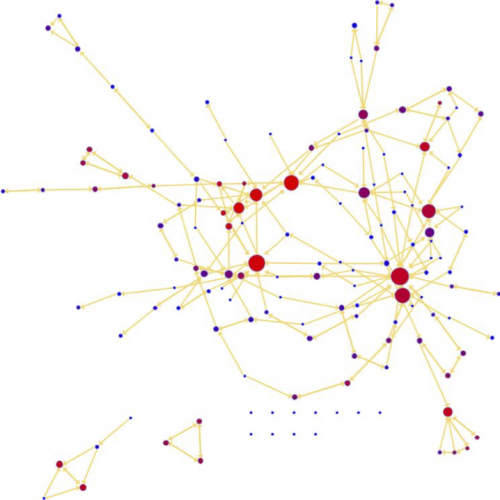
\includegraphics[scale=0.4]{ca}

\begin{small}\textit{\textbf{Figura 5.2}: Centralità del nodo rappresentato in una rete. I nodi più grandi (evidenziati in rosso) hanno valori di centralità più alti}.\end{small}
\end{center}

La definizione di \textit{centralità} varia a seconda del contesto o dello scopo dell'analisi che si sta eseguendo e può essere misurata utilizzando diverse metriche e criteri, per esempio:

\begin{enumerate}
\setlength{\itemsep}{1pt}
  \setlength{\parskip}{0pt}
  \setlength{\parsep}{0pt}
\item Il \textbf{grado dei nodi}.
\item Le \textbf{misure di centralità globale}. Due delle misure di centralità globale più utilizzate sono le centralità di \textit{prossimità} (\textit{closeness centrality}) e di \textit{interrelazione} (\textit{betweenness centrality}).\\

La \textit{closeness centrality} è una misura che stima la velocità del flusso di informazioni attraverso un dato nodo verso altri nodi. Essa misura quanto brevi sono i percorsi da un nodo verso tutti gli altri nodi.

La \textit{betweenness centrality} misura la frequenza con cui un nodo viene a trovarsi su tutti i percorsi più brevi fra due nodi\footnote{Questi nodi possono rappresentare proteine importanti nei percorsi di segnalazione e possono rappresentare obiettivi per la scoperta di farmaci. Combinando questi dati con l'analisi delle interferenze possiamo simulare attacchi mirati alle PPIN e prevedere quali proteine sono candidate migliori per la ricerca di farmaci.}.
\end{enumerate}

\subsection{\textit{Clustering Analysis}}
La ricerca di "comunità" all'interno di una rete è una buona strategia utile a ridurre la complessità della rete stessa e ad estrarre moduli funzionali (ad esempio, complessi proteici). I \textit{\textbf{cluster}} sono un gruppo di nodi che sono più connessi al loro interno che con il resto della rete. 

Quando si parla di PPIN, le comunità rientrano in due categorie: moduli funzionali e complessi proteici (si veda la \textit{\textbf{Sottosezione 3.3}} per la corretta definizione dei termini).

\subsubsection{Metodi di \textit{Clustering Analysis}}
Ora presentiamo brevemente due metodi che utilizzano esclusivamente la topologia della rete per individuare componenti strettamente connesse tra loro. Bisogna sottolineare che non si fanno ipotesi sulla struttura interna dei \textit{cluster}, concentreremo pertanto la nostra attenzione soltanto sulle regioni ad alta densità.

\begin{center}
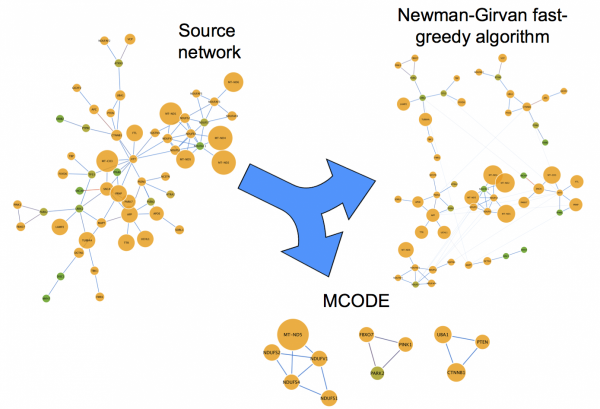
\includegraphics[scale=0.55]{ng}

\begin{small}\textit{\textbf{Figura 5.3}: Metodi di Clustering Analysis}.\end{small}
\end{center}

È importante notare che trovare la migliore struttura di "comunità" è algoritmicamente complesso ed è possibile solo per reti molto piccole. Per questo motivo sono stati sviluppati diversi metodi di approssimazione; ne presentiamo solamente due:
\begin{enumerate}
\item \textbf{Algoritmo \textit{Newman-Girvan fast-greedy}}: Questo metodo \textit{naïve} individua i \textit{cluster} grazie alla \textit{edge betweenness centrality measure}. Gli archi che collegano i diversi \textit{cluster} hanno \textit{centrality values} più elevate. Per definire i \textit{cluster} il metodo utilizza \textit{edge betweenness centrality scores} per classificare gli archi della rete, quindi rimuove gli archi più centrali e ricalcola i \textit{betweenness scores} fino a quando non rimangono più archi. Gli archi interessati dalla rimozione sono considerati parte dello stesso \textit{cluster}.
\item \textit{\textbf{Algoritmo MCODE}}: Questo metodo è stato appositamente sviluppato per trovare complessi proteici nelle PPIN. Più rigoroso dell'algoritmo Newman-Girvan, mira a trovare solo quelle sottoreti che sono altamente interconnesse (rappresentanti complessi proteici relativamente stabili, che funzionano come una singola entità nel tempo e nello spazio).
L'algoritmo utilizza un processo a tre fasi: (1) con il \textit{weighting} un punteggio più alto viene assegnato a quei nodi i cui vicini sono più interconnessi; (2) partendo dal nodo (denominato \textit{seed}) con il peso più elevato, vengono aggiunti al complesso i nodi che hanno un peso superiore ad una determinata soglia; (3) vengono applicati dei filtri per migliorare la qualità del \textit{cluster}.
\end{enumerate}

\section{PPIN: \textit{annotation enrichment analysis}}
Ci sono molti approcci diversi che possono essere utilizzati per comprendere il contesto biologico delle PPIN. L'\textit{annotation enrichment analysis} è uno dei metodi più popolari. Anche se non è propriamente uno strumento di analisi delle reti, è spesso utilizzato in combinazione con l'analisi topologica delle stesse.

Si utilizzano le annotazioni geniche/proteine fornite, per esempio, dall'Ontologia Genica (GO) per rispondere, attraverso un test statistico, alla seguente domanda:
\begin{center}
"Quando si campionano $X$ proteine (\textit{test set}) da $N$ proteine (\textit{reference set}; grafo o \textit{annotation}), qual è la probabilità che $x$, o più, di queste proteine appartengano ad una categoria funzionale $C$ condivisa da $n$ delle $N$ proteine nel \textit{reference set}?"
\end{center}
Il risultato di questo test ci fornisce una lista di termini che descrivono la rete (o una parte di essa) nel suo insieme, per identificare le "comunità" interconnesse trovate attraverso il \textit{topological clustering}.

I principali limiti dell'\textit{annotation enrichment analysis} derivano dalle \textit{annotation} stesse. Alcune aree della Biologia sono annotate più approfonditamente e meglio descritte di altre, con termini più dettagliati e più precisi (nel nostro caso, solo le proteine più "popolari" sono meglio annotate). Questo introduce una certa "distorsione" nell'analisi statistica.

È anche importante notare che i termini dell'Ontologia Genica (GO) possono essere assegnati sia da un curatore umano che esegue un'attenta annotazione manuale, sia da approcci computazionali che utilizzano le basi dell'annotazione manuale per dedurre quali termini descriverebbero in modo corretto i prodotti genici non scoperti. Ne consegue che un'altra limitazione è costituita dalla complessità e dal dettaglio dell'annotazione associati a grandi insiemi di geni o proteine. 
\pagebreak


Date due reti, \textbf{allinearle} significa trovare un mapping nodo-a-nodo (= \textit{alignement}) tra le reti in grado di ottimizzare due obiettivi: (1) massimizzare il numero di proteine mappate (corrispondenti ai nodi nel grafo) che sono correlate da un punto di vista funzionale e (2) massimizzare il numero di interazioni comuni (archi) tra le reti.

Il problema del \textit{Network alignment} è un problema intrattabile dovuto all'$\mathcal{NP}$-completezza sottostante al \textit{sub-graph isomorphism problem}\footnote{Problema computazionale nel quale, dati due grafi $G$ e $H$ in input, si vuole determinare se $G$ contiene un sottografo isomorfico ad $H$, deve cioè esistere una corrispondenza biunivoca tra gli elementi dei grafi.}, individuato da Spephen Cook nel 1971.

\section{MTGO}
Il metodo MTGO - \textit{Module detection via Topological information and GO knowledge} - costituisce un nuovo approccio di identificazione dei moduli funzionali nelle PPIN. Questo metodo combina le informazioni provenienti dalla topologia delle reti con la conoscenza biologica relativa alle proteine.
 
Per identificare i moduli più interessanti, MTGO utilizza partizioni ripetute della rete sfruttando la \textit{modularità} del grafo, corrispondente ad una funzione che misura la qualità topologica di una determinata partizione in un grafo. La partizione viene successivamente appresa attraverso un processo di ottimizzazione che tiene conto della struttura della rete e della sua natura biologica. A differenza dei precedenti approcci basati su GO, MTGO fornisce un unico termine GO che descrive al meglio la natura biologica di ogni modulo identificato.

Evidenziando i principali processi coinvolti nel sistema biologico, rappresentato dai modelli di PPIN, e grazie al suo modo unico di sfruttare l'Ontologia Genica, MTGO si differenzia in maniera significativa dagli algoritmi allo stato dell'arte (ClusterOne, MCODE -\textit{\textbf{Sottosezione 5.2.1}}-, COACH, CFinder, Markov Cluster MCL, DCAFP e GMFTP). 

Per valutare le performance di MTGO sono state selezionate, per i test, quattro PPIN reali: Krogan, Gavin, Collins e DIP Hsapi PPIN.\\

\begin{center}
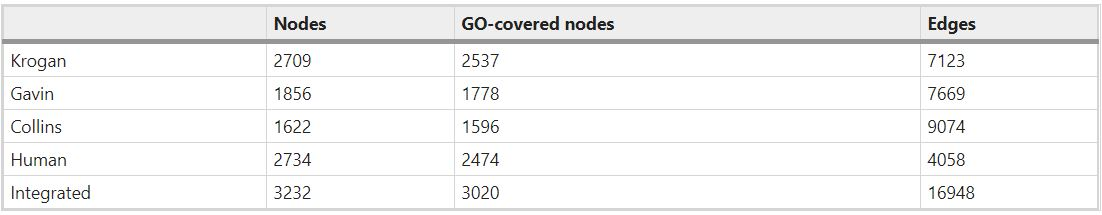
\includegraphics[scale=0.5]{tab1}

\begin{small}\textit{\textbf{Figura 7.1}: In questa tabella vengono indicate le caratteristiche principali di ogni rete, incluso il numero di nodi coperti dai termini GO, usati come input per MTGO}.\end{small}
\end{center}

I termini GO utilizzati come input per MTGO includono le seguenti tre categorie: \textit{Componente Cellulare}, \textit{Processo Biologico} e \textit{Funzione Molecolare}. 
MTGO ha mostrato i risultati migliori otto volte su nove ed è in grado di individuare complessi piccoli/sparsi anche in reti molto grandi.

MTGO è in grado di individuare moduli funzionali all'interno delle PPIN, prevede l'\textit{overlapping} e la copertura totale della rete\footnote{Si definisce \textit{copertura di nodi} (\textit{vertex cover}) di un grafo un insieme $C$ di nodi con la proprietà che ogni arco nel grafo abbia almeno uno dei suoi estremi in $C$.}, due \textit{features} importantissime per gli algoritmi di identificazione di moduli.

MTGO prevede una mappa sia dei moduli topologici che funzionali. I moduli topologici assicurano la copertura totale della rete, mentre quelli funzionali condividono i nodi, permettendo l'\textit{overlapping}; il metodo dipende fortemente dalla qualità dei termini GO, le sue performance infatti diminuiscono significativamente a seconda della perturbazione (del 25\%, 50\% e 75\%) dei termini GO forniti ed è stato progettato per essere testato sia su reti pesate che non. 

MTGO possiede l'abilità di individuare un insieme di termini GO fornendo un'interpretazione biologica significativa della PPIN, proprietà assente negli altri algoritmi allo stato dell'arte.\\

\begin{center}
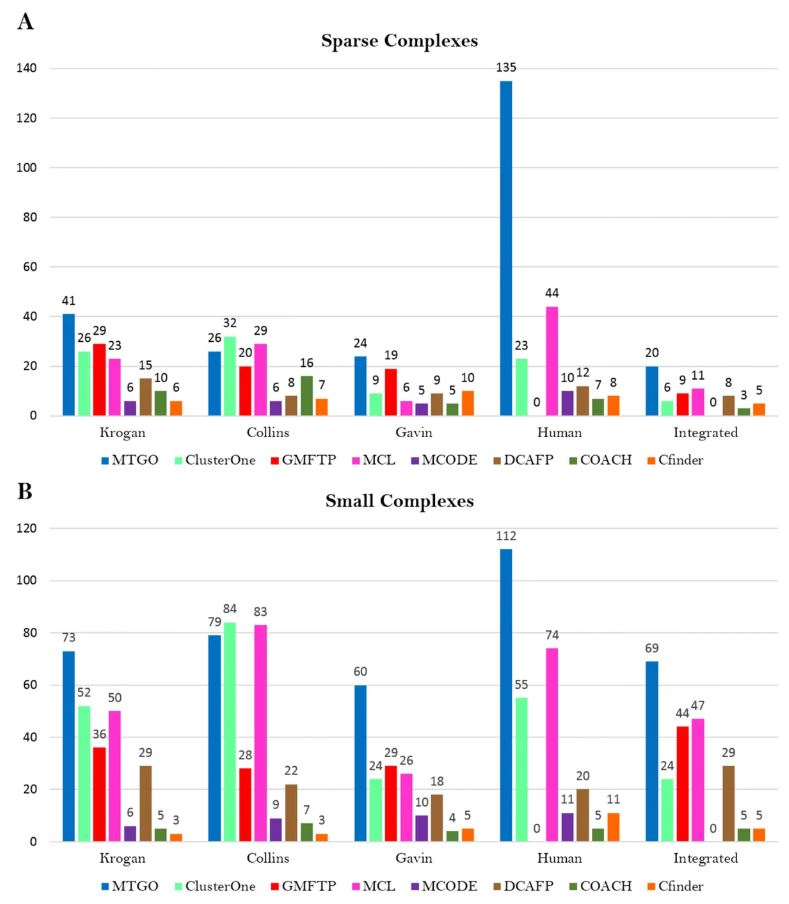
\includegraphics[scale=0.65]{prest1}

\begin{small}\textit{\textbf{Figura 7.2}: Confronto di MTGO con gli altri metodi}.\end{small}
\end{center}

\subsection{MTGO: inizializzazione, iterazioni e convergenza}
Una PPIN può essere rappresentata tramite un grafo $G = (V,E)$ dove $V$ ed $E$ corrispondono ai nodi e agli archi della rete, rispettivamente. $V$ è l'insieme delle proteine ed è definito come $V =\left \{v_1, v_2, v_3, ..., v_N\right \}$ dove $N$ è il numero di proteine/nodi totale. $E$ rappresenta l'insieme delle relazioni tra i nodi della rete: $E = \left \{e_{i,j}\right \}$, $(i,j) \in$ [1,$N$]. Inoltre, $G$ detiene le proprietà topologiche PPI. Per integrare le informazioni relative alle funzioni biologiche all'interno della rete, ai nodi vengono associati i termini GO. MTGO calcola l'insieme $T = (L, \Delta)$, dove il $p$-esimo elemento è $t_p = (l_p, \delta_p)$, $l_p$ rappresenta l'\textit{ontology term}, mentre $\delta_p$ è l'$l_p$-insieme associato alla rete di proteine (si veda la \textit{\textbf{Figura 7.3}} per un esempio).

\begin{center}
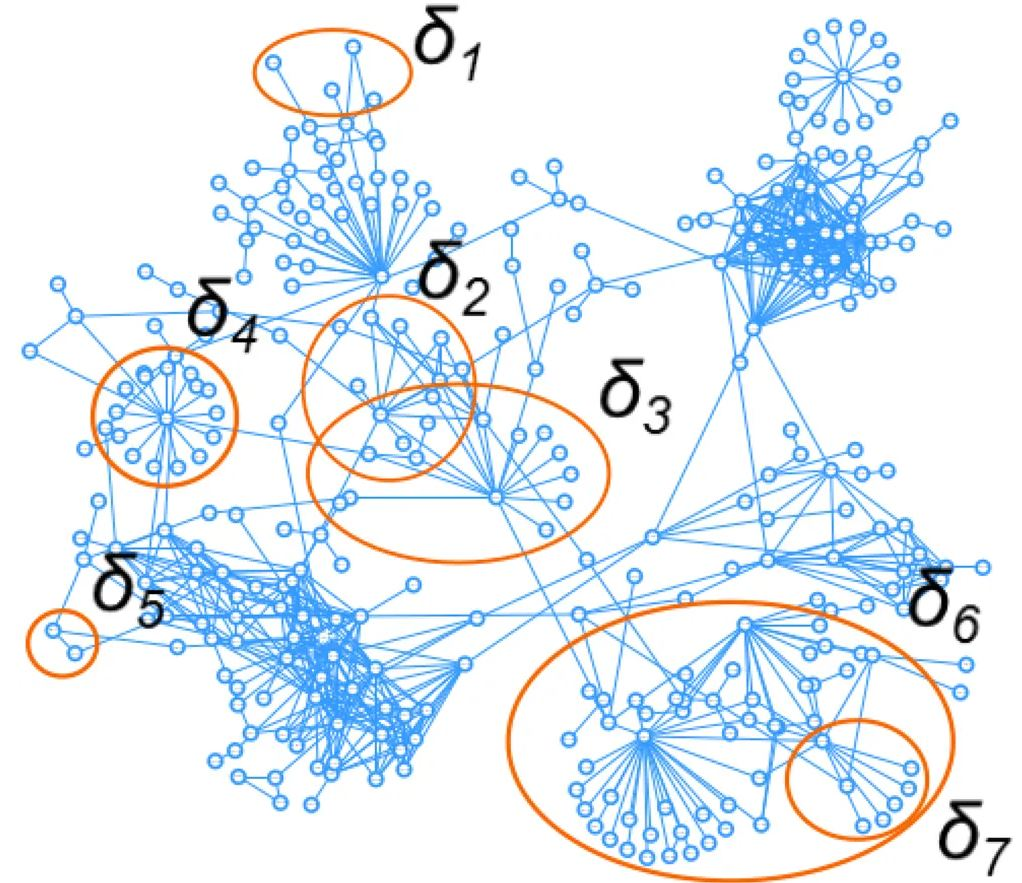
\includegraphics[scale=0.35]{delta}

\begin{small}\textit{\textbf{Figura 7.3}: Esempio dei $\delta$ elementi rappresentati in una rete, potrebbero condividere più nodi o essere inclusi in una categoria più vasta}.\end{small}
\end{center}

$I = (G,T)$ è l'input del sistema. L'obiettivo di MTGO è quello di processare $G$ per trovare gruppi di nodi che condividono sia le proprietà topologiche $(V,E)$, sia quelle funzionali $(T)$. L'output di questo metodo è $R^F = (C^F, \Phi^F)$ dove $C^F$ è l'insieme dei moduli topologici, mentre $\Phi^F$ è l'insieme dei moduli funzionali. Da notare che $|C^F| = |\Phi^F|$, la relazione è 1:1. 

MTGO calcola iterativamente $C$ e $\Phi$ e la coppia $R^F = (C^F, \Phi^F)$ viene selezionata come output finale.

L'insieme di moduli topologici $C$ costituisce una partizione della rete, $C = \left \{c_1, ..., c_h, ..., c_H\right \}$, di modo che:

\begin{center}
$c_1 \cap c_2 ... \cap c_h ... \cap c_H \equiv \emptyset$
\end{center}
\begin{center}
 $c_1 \cup c_2 ... \cup c_h ... \cup c_H \equiv V$.
\end{center}

Bisogna notare che ogni nodo di una partizione di $C$ viene unicamente assegnata ad un singolo modulo topologico. D'altra parte, l'insieme $\Phi = \left \{\phi_1, ..., \phi_h, ..., \phi_H\right \}$ descrive i moduli funzionali coinvolti nella rete. $\Phi$ viene definito in questo modo:

\begin{center}
$\phi_1 \cap \phi_2 ... \cap \phi_h ... \cap \phi_H \equiv \emptyset$
\end{center}
\begin{center}
 $\phi_1 \cup \phi_2 ... \cup \phi_h ... \cup \phi_H \subseteq V$
\end{center}

e $\Phi \subset T$, cioè $\Phi$ è il sottoinsieme di $T$ selezionato da MTGO per descrivere le funzioni biologiche collegate alla partizione $C$ della PPIN.

La copertura completa (\textit{full coverage}) e la sovrapposizione (\textit{overlapping}) sono considerate le caratteristiche ideali degli algoritmi di identificazione di moduli. MTGO garantisce entrambe queste proprietà con il suo doppio output complementare $C$ e $\Phi$. In particolare, i moduli topologici $C$ rappresentano una partizione di rete, garantendo una copertura completa per definizione. I moduli funzionali $\Phi$ si sovrappongono, consentendo l'assegnazione di un nodo a due o più moduli. Questa caratteristica è particolarmente importante in quanto riflette il comportamento dei sistemi biologici, dove una proteina può essere coinvolta in molteplici funzioni.\\

Vediamo ora di capire, per lo meno a livello intuitivo, i passi eseguiti da MTGO.
Dato l'input $I = (G,T)$, MTGO realizza tre fasi principali: (1) inizializzazione, (2) iterazione e (3) controllo della convergenza.

\begin{center}
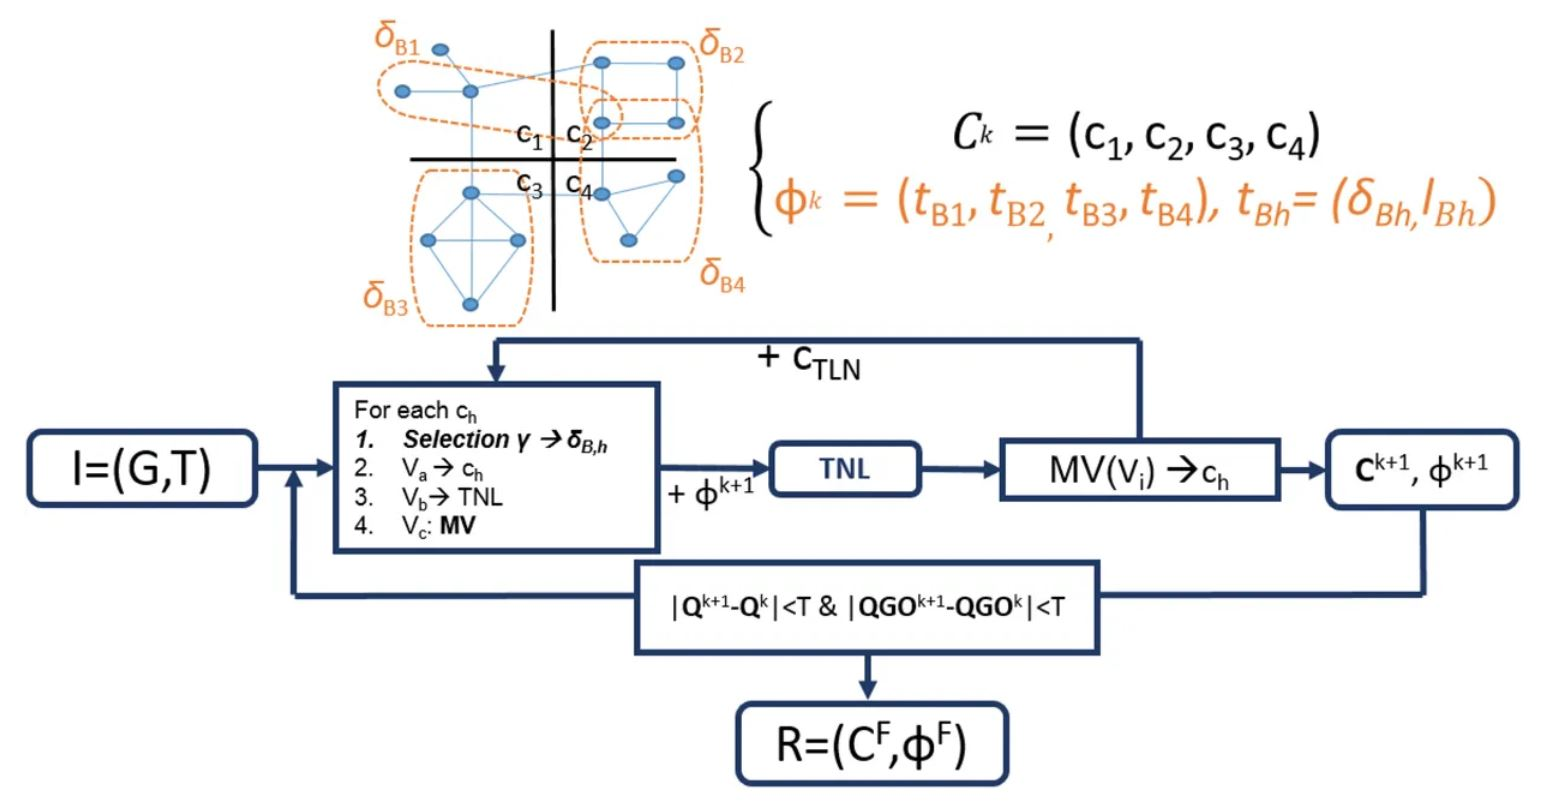
\includegraphics[scale=0.37]{algMTGO}

\begin{small}\textit{\textbf{Figura 7.4}: Rappresentazione dei passi seguiti dall'algoritmo MTGO}.\end{small}
\end{center}

Nella fase di \textbf{inizializzazione}, $V$ viene utilizzato per generare una partizione casuale $C^0$ nella quale il numero di moduli topologici è $\propto \sqrt{N}$. $T$ viene creato partendo da una \textit{GO term list} fornita dall'utente (in conformità all'insieme $V$). Vengono successivamente definiti, sempre dall'utente, due parametri ($minSize$ e $maxSize$) che definiscono la minima e la massima taglia dei moduli in $T$, cioè il numero di nodi in un $\delta_p$.

\begin{center}
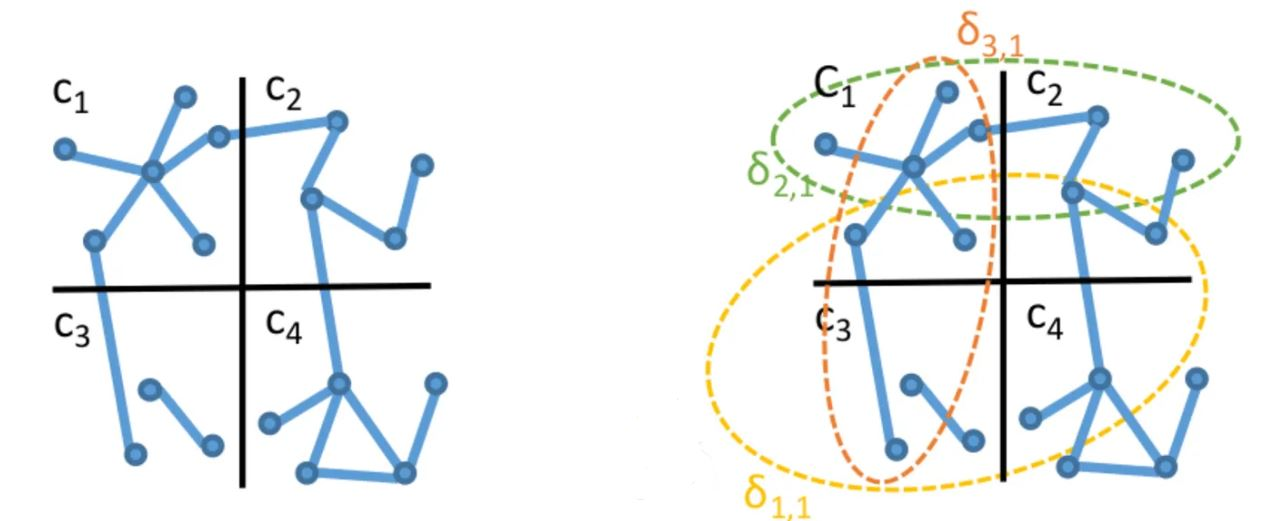
\includegraphics[scale=0.38]{deltax}

\begin{small}\textit{\textbf{Figura 7.5}: Le fasi di MTGO}.\end{small}
\end{center}

Ad ogni \textbf{iterazione} viene calcolata una coppia $(C, \Phi)$, in particolare $C$ ri-assegnando i nodi alla partizione precedente e $\Phi$ selezionando elementi da $T$ che descrivono al meglio $C$. Ogni partizione di $C$ è costituita da $c_h$ moduli topologici con $h$ rappresentante l'indice di una singolo modulo topologico ($1\leq h \leq H$, il numero totale dei moduli funzionali $H$ varia ad ogni iterazione). Idealmente, MTGO tende ad assegnare i nodi in modo che i moduli topologici coincidano con quelli funzionali\footnote{Per una trattazione dettagliata di questa fase rimandiamo alla lettura delle due sottofasi descritte nel dettaglio nel paper di riferimento (si veda la \textbf{Bibliografia}).}).

\begin{center}
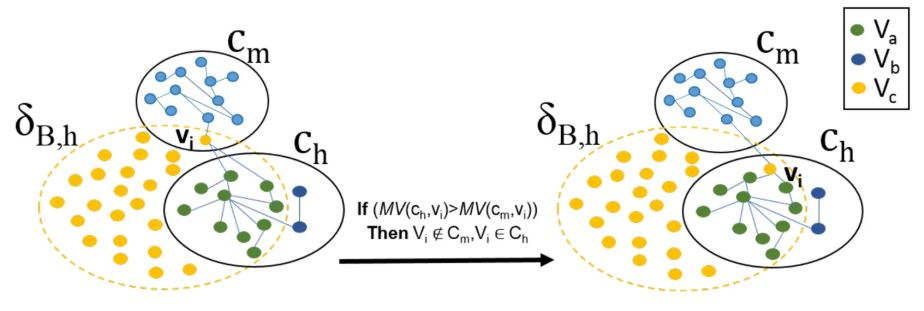
\includegraphics[scale=0.62]{deltaa}

\begin{small}\textit{\textbf{Figura 7.6}: Riassegnamento di un nodo}.\end{small}
\end{center}

Per valutare se la \textbf{convergenza} è stata raggiunta o meno si utilizzano due funzioni: \textit{modularità} ($Q$) e \textit{Quality GO} ($QGO$): $Q$ valuta la qualità globale della partizione $C$, $QGO$ valuta la corrispondenza e il conseguente \textit{overlapping} tra $C$ e $\Phi$. Idealmente, $C$ e $\Phi$ dovrebbero essere soggette ad \textit{overlapping}.

La formula di $Q$ è:

\begin{center}
$Q(C^k) = \displaystyle{\sum_{1<h<H_k}\frac{e^k_h}{|E|} - \left(\frac{d^k_h}{2 \times |E|}\right)^2}$
\end{center}

Questa formula serve a valutare le partizioni dei grafi. L'indice $k$ indica la $k$-esima iterazione dell'algoritmo. $C^k$ è la $k$-esima partizione, $H^k$ è il numero di moduli topologici, $e^k_h$ è il numero totale di archi nell'$h$-esimo modulo topologico mentre $d^k_h$ è la somma dei gradi dei nodi dell'$h$-esimo modulo topologico. 

Il valore di $Q$ varia da -1 a 1, i valori positivi (negativi) indicano un maggior (minor) numero di collegamenti all'interno dei moduli topologici rispetto ad una randomizzazione.\\

MTGO rimane, a quasi 3 anni dallo sviluppo, sconosciuto ai più con solamente 13 citazioni su Google Scholar. Dato comunque l'esiguo numero di citazioni, questo metodo rimane il metro di paragone utilizzato da altri ricercatori nello sviluppo di efficienti algoritmi per l'identificazione di moduli funzionali nelle PPIN.

\pagebreak
\section{IsoRank}
IsoRank è un metodo per l'allineamento globale di più PPIN. L'intuizione da tener presente è che una proteina in una rete PPI produce una buona corrispondenza (\textit{match}) con una proteina in un'altra rete se le loro rispettive sequenze e i loro intorni topologici costituiscono una buona corrispondenza. IsoRank è stato utilizzato per calcolare un allineamento globale delle reti PPI \textit{Saccharomyces cerevisiae} (lievito di birra -fungo-), \textit{Drosophila melanogaster} (moscerino della frutta), \textit{Caenorhabditis elegans} (verme), \textit{Mus musculus} (topo comune) e \textit{Homo sapiens}.

I sottografi individuati con questi allineamenti sono più grandi e più vari di quelli prodotti da metodi precedenti che hanno dimostrato la loro efficacia nell'identificare pattern localizzati confrontando tra di loro solamente due reti. Questo metodo rappresenta un grande passo avanti per l'allineamento di più reti PPI ed è applicabile in molti settori scientifici.

IsoRank rappresenta un approccio di analisi comparativa delle reti PPI al fine di trovare una soluzione al problema di allineamento ottimo \textit{globale} tra due o più PPIN, mirando a trovare la corrispondenza tra i nodi e gli archi delle reti in input che massimizzi il \textit{match} totale tra le reti.

\subsection{\textit{Global} vs. \textit{Local Network Alignment}}
In generale, l'obiettivo in un problema di allineamento di rete è quello di trovare un sottografo comune (cioè un insieme di archi "conservati") tra le reti in input. Corrispondentemente a questi archi conservati, esiste una mappatura (\textit{mapping}) tra i nodi delle reti. Per esempio, quando la proteina $a_1$ dalla rete $G_1$ viene mappata sulle proteine $a_2$ in $G_2$ e $a_3$ in $G_3$, allora $a_1$, $a_2$ e $a_3$ si riferiscono allo stesso nodo nell'insieme degli archi conservati. Ciò che rende difficile il problema è il compromesso (\textit{trade-off}) da ottenere: massimizzare la sovrapposizione (\textit{overlap}) tra le reti (cioè il numero di archi conservati), garantendo al tempo stesso che le proteine mappate siano il più possibile correlate.

Mentre un algoritmo \textit{Local Network Alignment} è essenzialmente destinato a trovare pattern simili tra due reti (o sottoreti), l'obiettivo nel \textit{Global Network Alignment} è quello di trovare il miglior allineamento complessivo tra le reti in ingresso.
Inoltre, deve valere una proprietà di \textit{transitività}: se $a_1$ in $G_1$ viene mappata su $a_2$ in $G_2$ e $a_2$ viene mappata su $a_3$ e $a_4$ in $G_3$, allora anche $a_1$ dovrebbe essere mappata su $a_3$ e $a_4$. Il GNA può essere usato per confrontare gli interattomi e per comprendere le variazioni tra specie.

\subsection{\textit{Score} e \textit{mapping}}
Consideriamo un semplice caso di GNA a coppie. L'input consiste in due PPIN $G_1$ e $G_2$ (ogni arco $e$ può aver associato un peso $w(e)$, con $0\leq w(e) \leq1$) e di una \textit{similarity measure} tra i nodi delle due reti (per esempio BLAST \textit{similarity measure}).

L'output desiderato è un mapping tra i nodi delle due reti che massimizza la combinazione convessa delle seguenti funzioni obiettivo: (1) la dimensione del grafo in comune in seguito al mapping e (2) la somiglianza tra le sequenze dei nodi mappati gli uni negli altri.

L'algoritmo prevede \textbf{due fasi}. Nella prima fase associa un \textit{functional similarity score} ad ogni possibile match tra i nodi delle due reti. Sia $R_{ij}$ lo \textit{score} per la coppia di proteine ($i,j$) dove $i$ proviene dalla rete $G_1$, mentre $j$ da $G_2$. La seconda fase costruisce la mappatura per il GNA estraendo un insieme di \textit{score} elevati (in accordo con \textit{\textbf{R}}, il vettore di tutti $R_{ij}$).
Per calcolare il \textit{functional similarity score} $R_{ij}$ consideriamo la coppia ($i,j$) un "buon match" se le sequenze di $i$ e di $j$ sono allineate e i loro "vicini" costituiscono a loro volta un buon match gli uni con gli altri. Bisogna quindi generare un insieme di vincoli e calcolare i \textit{neighborhood scores} in modo ricorsivo. Si consideri la seguente equazione:

\begin{center}
\textit{\textbf{R}} = $\sum R_{ij}$ = $\displaystyle{\sum_{u \in N(i)}} \displaystyle{\sum_{v \in N(j)}\frac{1}{|N(i)||N(j)|} R_{ij}}$ con $i \in V_1$, $j \in V_2$
\end{center}

dove $N(a)$ rappresenta tutti i \textit{neighbors} del nodo $a$; $|N(a)|$ la cardinalità di questo insieme; $V_1$ e $V_2$ sono gli insiemi dei nodi nelle reti $G_1$ e $G_2$ rispettivamente. Lo \textit{score} $R_{ij}$ dipende dagli \textit{score} dei vicini di $i$ e $j$, che a loro volta dipendono dai vicini dei vicini etc.

I nodi che hanno una buona corrispondenza hanno valori score $R_{ij}$ più alti.

\begin{center}
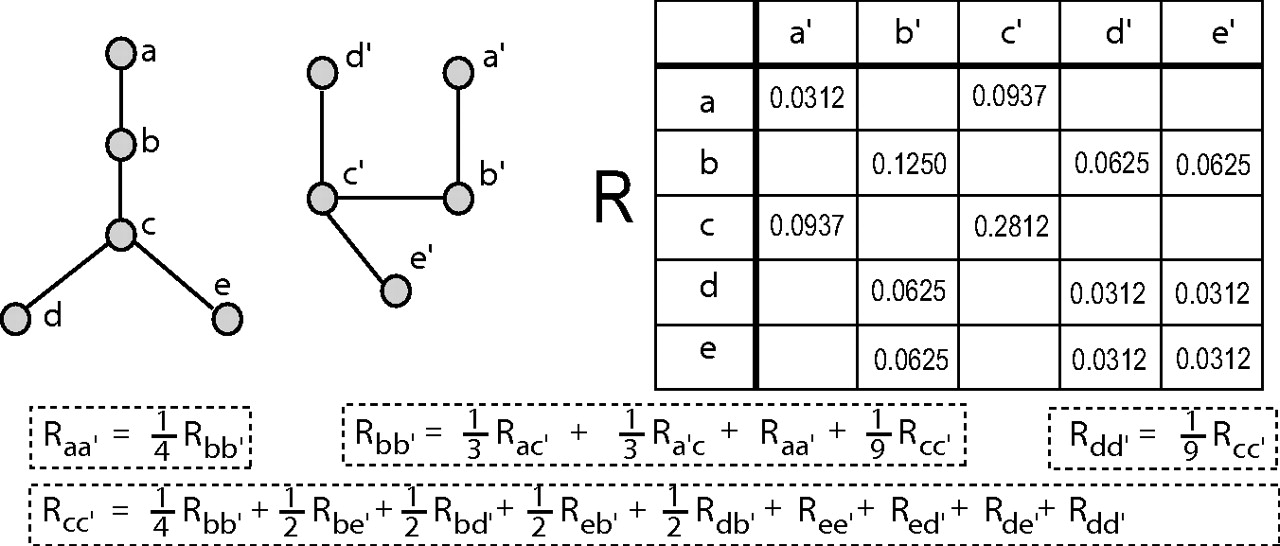
\includegraphics[scale=0.3]{isorank}

\begin{small}\textit{\textbf{Figura 8.1}: Intuizione alla base dell'algoritmo: consideriamo una coppia di grafi isomorfi di piccole dimensioni; per ogni possibile accoppiamento $(i,j)$ tra i nodi dei due grafi calcoliamo i valori $R_{ij}$. Questi valori sono vincolati (\textit{constrained}) a dipendere dai valori dei "vicini" (si veda l'equazione)}.\end{small}
\end{center}

A questo punto dell'algoritmo abbiamo uno score $R_{ij}$ per ogni coppia di nodi che non sono nella stessa rete; in genere, per il 99\% delle coppie-nodo, questo valore è zero. Dopo aver identificato gli score più alti bisogna assicurarsi che il \textit{mapping} mantenga la proprietà di transitività (descritta in precedenza). Il \textit{mapping} si può ottenere in due modi: 
\begin{enumerate}
\setlength{\itemsep}{1pt}
  \setlength{\parskip}{0pt}
  \setlength{\parsep}{0pt}
\item \textbf{One-to-one Mapping}: ogni nodo viene mappato in al massimo un altro nodo (per specie);
\item \textbf{Many-to-many}: un nodo può essere mappato in più di un nodo in un'altra specie.\footnote{\textbf{Multiple GNA}: Quando l'input consiste di più di due reti, si ripete il processo appena descritto per tutte le possibili coppie di reti fornite in input e successivamente si calcolano i \textit{functional similarity scores} \textit{\textbf{R}} per ogni coppia di reti in input.}
\end{enumerate}

Concludiamo proponendo l'analisi del sottografo comune ottenuto dall'allineamento delle cinque specie elencate in precedenza.

Il sottografo corrispondente all'allineamento globale possiede 1663 archi in comune ad almeno due PPIN e 157 archi in comune al almeno 3 PPIN. La dimensione del sottografo comune è relativamente piccola (\textit{overlap} solamente con $\approx$ 5\% della PPIN umana) a causa delle probabili incompletezza e rumorosità dei dati. All'aumentare della quantità e della qualità dei dati, l'\textit{overlap} dovrebbe aumentare sensibilmente. Delle 86932 proteine provenienti dalle 5 specie, 59539 (68,5\%) hanno ottenuto almeno un match con un'altra proteina di una rete diversa.\\

IsoRank è stato citato ben 505 volte (fonte: Google Scholar) dallo sviluppo nel 2008, proposto in moltissime varianti, costituisce un "baluardo" per il GNA.

\pagebreak
\section{\textit{struc2vec}}
La \textit{structural identity} (traducibile con \textit{identità strutturale}) corrisponde ad un concetto di simmetria nel quale i nodi di una rete vengono identificati in base alla struttura della rete stessa e tramite relazioni con altri nodi. \\

\textit{struc2vec} è un framework flessibile per l'apprendimento di \textit{latent representations} (= tutte le informazioni importanti necessarie per rappresentare i dati originali) per l'identità strutturale dei nodi\footnote{Nodi che hanno \textit{neighborhoods} con insiemi simili di nodi dovrebbero avere \textit{latent representations} simili. Ma il \textit{neighborhood} è un concetto locale definito da una nozione di "prossimità" nella rete. Per questo motivo, due nodi "vicini" che sono strutturalmente simili ma molto distanti nella rete avranno \textit{latent representations} diverse. Si veda la \textit{\textbf{Figura 9.1}}.}. \textit{struc2vec} utilizza una gerarchia, definita dalla sequenza ordinata dei gradi dei nodi, per misurare la \textit{similarity} dei nodi stessi e costruisce un grafo multi-livello (\textit{multilayer graph}) per codificare le somiglianze strutturali.

Sviluppato nel 2017, \textit{struc2vec} presenta prestazioni molto elevate nell'acquisizione di nozioni di identità strutturale in quanto supera i limiti raggiunti dagli approcci precedenti. Gli esperimenti numerici indicano che \textit{struc2vec} migliora le prestazioni su attività di classificazione che dipendono principalmente dall'identità strutturale; \textit{struc2vec} eccelle anche quando la rete originale è soggetta a forti rumori casuali (e.g. rimozione casuale di archi dal grafo).

In quasi tutte le reti, i nodi tendono ad avere una o più funzioni che determinano il loro ruolo nel sistema; come abbiamo imparato, le proteine in una rete di interazione proteina-proteina (PPIN) esercitano funzioni specifiche. 
Intuitivamente, dunque, diversi nodi in tali reti possono eseguire funzioni simili e spesso possono essere partizionati in classi equivalenti rispetto alla loro funzione nella rete.

\begin{center}
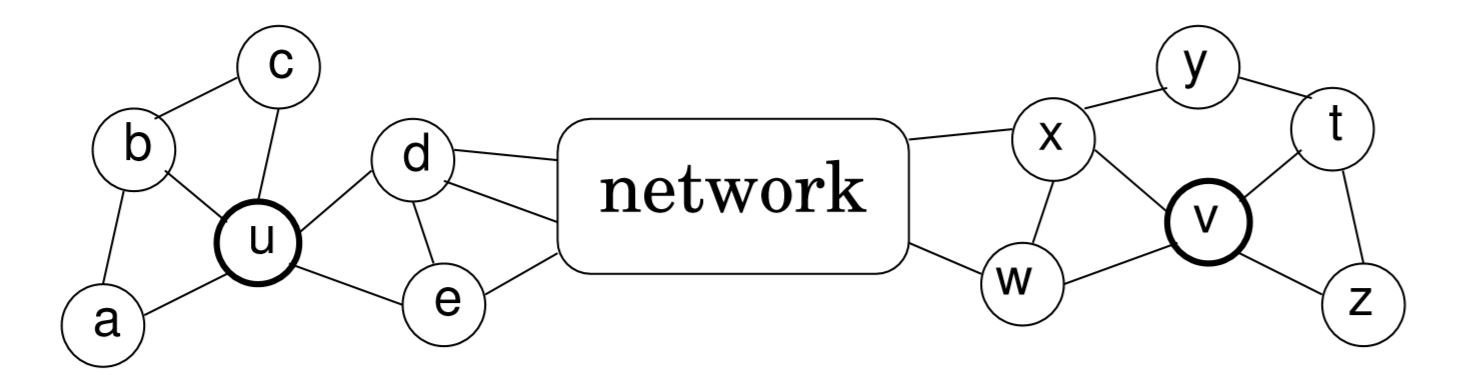
\includegraphics[scale=0.36]{struc1}

\begin{small}\textit{\textbf{Figura 9.1}: Esempio di due nodi (u e v) strutturalmente simili (gradi 5 e 4, connessi a 3 e 2 triangoli, collegati al resto della rete da due nodi), ma molto distanti nella rete}.\end{small}
\end{center}

\subsection{\textit{struc2vec}: idee di base}
Elenchiamo qui di seguito le idee fondamentali che stanno alla base di questo metodo:
\begin{enumerate}
\setlength{\itemsep}{1pt}
  \setlength{\parskip}{0pt}
  \setlength{\parsep}{0pt}
  \item Valuta la \textit{structural similarity} tra i nodi indipendentemente da eventuali attributi associati a nodi o archi, o addirittura dalla loro posizione all'interno della rete. Due nodi che hanno una struttura locale simile saranno considerati "strutturalmente simili", indipendentemente dalla posizione di rete e dai \textit{labels} associati ai vari \textit{neighborhoods}.
  
Questo approccio inoltre non richiede un grafo connesso, identifica nodi strutturalmente simili anche in componenti connesse diverse.
  \item Stabilisce una gerarchia per valutare la \textit{structural similarity}.
Ai livelli inferiori della gerarchia la \textit{structural similarity} tra i nodi dipende solamente dai loro gradi, per poi, man mano che si procede verso la cima, dipendere dall'intera rete (dal punto di vista del nodo).
  \item Genera sequenze di nodi strutturalmente simili  (in seguito ad una \textit{random walk} pesata che attraversa un grafo multilayer (e non la rete originale). Pertanto, due nodi che appaiono frequentemente con sequenze simili avranno molto probabilmente una struttura simile.
\end{enumerate}

Consideriamo ora il problema delle \textit{learning representations} che catturano l'identità strutturale dei nodi nella rete. Un approccio corretto dovrebbe presentare queste due proprietà:
\begin{itemize}
\setlength{\itemsep}{1pt}
  \setlength{\parskip}{0pt}
  \setlength{\parsep}{0pt}
  \item La distanza tra la \textit{latent representation} dei nodi dovrebbe essere fortemente correlata alla loro somiglianza strutturale. Per questo motivo, due nodi con strutture di rete locale identiche dovrebbero anche avere la stessa \textit{latent representation}, mentre i nodi con identità strutturali diverse dovrebbero essere lontani fra loro.
  \item La \textit{latent representation} non deve dipendere da alcun attributo di nodi o archi, inclusi i \textit{labels} dei nodi. Dunque, nodi strutturalmente simili devono avere una rappresentazione latente stretta, indipendente dagli attributi del nodo e degli archi nel proprio \textit{neighborhood}.
L'identità strutturale dei nodi deve essere indipendente dalla sua "posizione" nella rete.
\end{itemize}

Tenendo presente queste due proprietà, \textit{struct2vec} può essere suddiviso in quattro step principali:
\begin{enumerate}
\setlength{\itemsep}{1pt}
  \setlength{\parskip}{0pt}
  \setlength{\parsep}{0pt}
  \item Determinazione della somiglianza strutturale tra ogni coppia di vertici nel grafo per dimensioni di \textit{neighborhood} diverse; questo fatto porta alla generazione di una gerarchia che fornisce maggiori informazioni per valutare la somiglianza strutturale ad ogni livello della stessa.
  \item Costruzione di un grafo multi-livello pesato in cui tutti i nodi della rete compaiono in ogni layer e ogni layer corrisponde ad un livello della gerarchia nella misurazione della \textit{structural similarity}.
  \item Utilizzo del grafo multi-livello per generare (tramite \textit{random walks}) sequenze di nodi. È probabile che queste sequenze includano nodi che sono più strutturalmente simili di altri.
  \item Data la sequenza di nodi, apprendimento della \textit{latent representation}.
\end{enumerate}

\subsection{\textit{struc2vec}: descrizione delle iterazioni}
Il primo passo compiuto dall'algoritmo consiste nel determinare l'identità strutturale tra due nodi senza utilizzare attribuiti di nodi o di archi. Intuitivamente, due nodi che hanno lo stesso grado sono strutturalmente simili, ma se i loro vicini hanno anch'essi lo stesso grado, allora sono ancora di più strutturalmente simili.\\

Sia $G = (V,E)$ un grafo non orientato e non pesato dove $V$ è l'insieme dei vertici ed $E$ quello degli archi, dove $n = |V|$ indica in numero dei nodi e $k^*$ il diametro (= la più grande distanza tra coppie di nodi del grafo). Sia $R_k(u)$ l'insieme dei nodi a distanza esattamente $k \geq 0$ da $u$ in $G$. $R_1(u)$ denota l'insieme dei vicini di $u$ e in generale $R_k(u)$ denota l'anello di nodi distanti $k$. Sia $s(S)$ la sequenza ordinata di gradi di un \textit{set} $S \subset V$ di nodi. Comparando le sequenze di gradi ordinate degli anelli a distanza $k$ fra $u$ e $v$ possiamo indicare con $f_k(u,v)$ la \textit{structural distance} tra $u$ e $v$ considerando i loro $k$-hop \textit{neighborhoods} (tutti i nodi a distanza minore o uguale a $k$ e tutti gli archi tra di loro). In particolare, definiamo:
\begin{center}
$f_k(u,v) = f_{k-1}(u,v) + g(s(R_k(u)),s(R_k(v)))$, 
\end{center}
\begin{center}
$k \geq 0$ e $|R_k(u)|, |R_k(v)| > 0$
\end{center}
dove $g(D_1,D_2) \geq 0$ misura la distanza tra le sequenze ordinate $D_1$ e $D_2$. 

Per confrontare i gradi di due sequenze si utilizza \textit{Dynamic Time Warping}\footnote{Algoritmo che permette l'allineamento tra due sequenze, e che può portare ad una misura di distanza tra le due sequenze allineate.}. DTW trova l'allineamento ottimo fra due sequenze $A$ e $B$. Data una funzione distanza $d(a,b)$ per gli elementi della sequenza, DTW confronta ogni elemento $a \in A$ e $b \in B$, di modo che la somma delle distanze tra elementi corrispondenti (\textit{matched}) sia minima. Dal momento che gli elementi delle sequenze $A$ e $B$ sono i gradi dei nodi, viene adottata la seguente formula:
\begin{center}
$d(a,b) = \displaystyle{\frac{max(a,b)}{min(a,b)}}-1$
\end{center}

Notare che quando $a = b$ allora $d(a,b) = 0$. Per questo motivo due sequenze ordinate di gradi, identiche, avranno distanza pari a 0.\\

A questo punto è necessario costruire un grafo a più strati pesato che codifichi la \textit{structural similarity} tra i nodi. 

Sia $M$ questo grafo dove il layer $k$ viene definito utilizzando i $k$-hop \textit{neighborhoods} dei nodi. Ogni layer $k = 0,...,k^*$ è formato da un grafo non orientato completo e pesato con $V$ insieme dei nodi e $\displaystyle{\left(\frac{n}{2}\right)}$ archi. Il peso dell'arco tra due nodi in un layer è dato dalla seguente formula:
\begin{center}
$w_k(u,v) = e^{-f_k(u,v)}$, $k = 0,...,k^*$
\end{center}
I nodi che saranno strutturalmente simili a $u$ avranno pesi maggiori tra i vari layer di $M$. I layer vengono collegati utilizzando archi orientati: ogni vertice è collegato al corrispondente nei layer superiore ed inferiore. Perciò, ogni vertice $u \in V$ nel layer $k$ è collegato al corrispondente vertice $u$ nei layer $k+1$ e $k-1$. Il peso degli archi tra i layer è definito in questo modo:
\begin{center}
$w(u_k,u_{k+1}) = log(\Gamma_k(u) + e)$, $k = 0,...,k^*-1$
\end{center}
\begin{center}
$w(u_k,u_{k-1}) = 1$, $k = 1,...,k^*$
\end{center}
dove $\Gamma_k(u)$ è il numero di archi incidenti in $u$ che hanno peso maggiore del peso medio di un arco nel grafo completo al layer $k$. In particolare:
\begin{center}
$\Gamma_k(u) = \displaystyle{\sum_{v \in V}} \mathbb{I}(w_k(u,v) > \bar w_k)$
\end{center}
misura la \textit{similarity} tra il nodo $u$ e gli altri nodi nel layer $k$.
Per ogni nodo $u$ \textit{struc2vec} procede con una \textit{random walk} partendo dal layer 0. Queste \textit{random walk} hanno una lunghezza (= numero di passi) fissata e relativamente corta; il processo viene ripetuto un certo numero di volte, dando luogo a \textit{walks} multiple ed indipendenti.

Si utilizza infine \textit{Skip-Gram}, una tecnica di \textit{unsupervised learning} per NLP, per identificare o derivare le \textit{latent representations} dalle sequenze ottenute.\\

A \textit{struc2vec} è possibile applicare una serie di ottimizzazioni (a partire dall'implementazione di DTW, che raggiunge una complessità di $O(l)$ a fronte dell'$O(l^2)$ iniziale) che permettono di raggiungere una complessità di $O(k^*n^3)$ grazie alla riduzione della lunghezza delle sequenze dei gradi e del numero dei layer.\\

\textit{struc2vec} è stato testato in diversi scenari e confrontato con gli algoritmi allo stato dell'arte (\textit{DeepWalk} e \textit{node2vec}) per l'apprendimento di \textit{latent representations}.

Il primo test ha previsto la costruzione di un particolare tipo di grafo, denominato \textit{barbell graph}, costituito da due grafi completi connessi da un \textit{path graph}. Ogni coppia di nodi che è strutturalmente equivalente dovrebbe avere \textit{latent representations} simili (che a loro volta dovrebbero essere in grado di descrivere, nel miglior modo possibile, la gerarchia strutturale).

\begin{center}
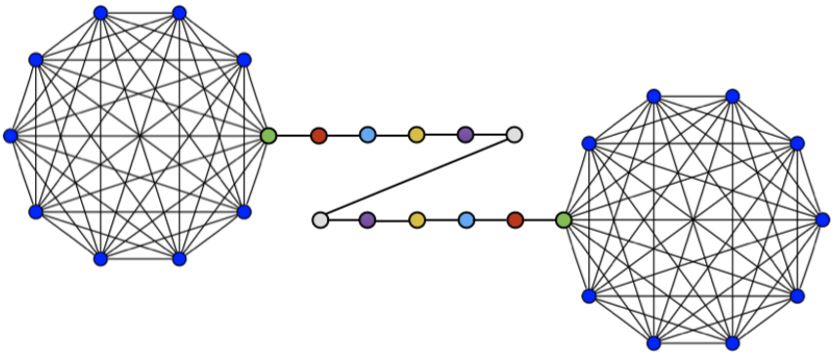
\includegraphics[scale=0.6]{struc6}

\begin{small}\textit{\textbf{Figura 9.2}: Barbell graph}.\end{small}
\end{center}

Anche in seguito ad un tuning dei parametri, \textit{DeepWalk} fallisce nell'individuare le equivalenze strutturali, mentre \textit{node2vec} non riconosce le identità strutturali; \textit{struc2vec} invece individua le \textit{latent representations} posizionando inoltre i nodi strutturalmente equivalenti gli uni vicino agli altri (si veda la \textit{\textbf{Figura 9.3}}).

\begin{center}
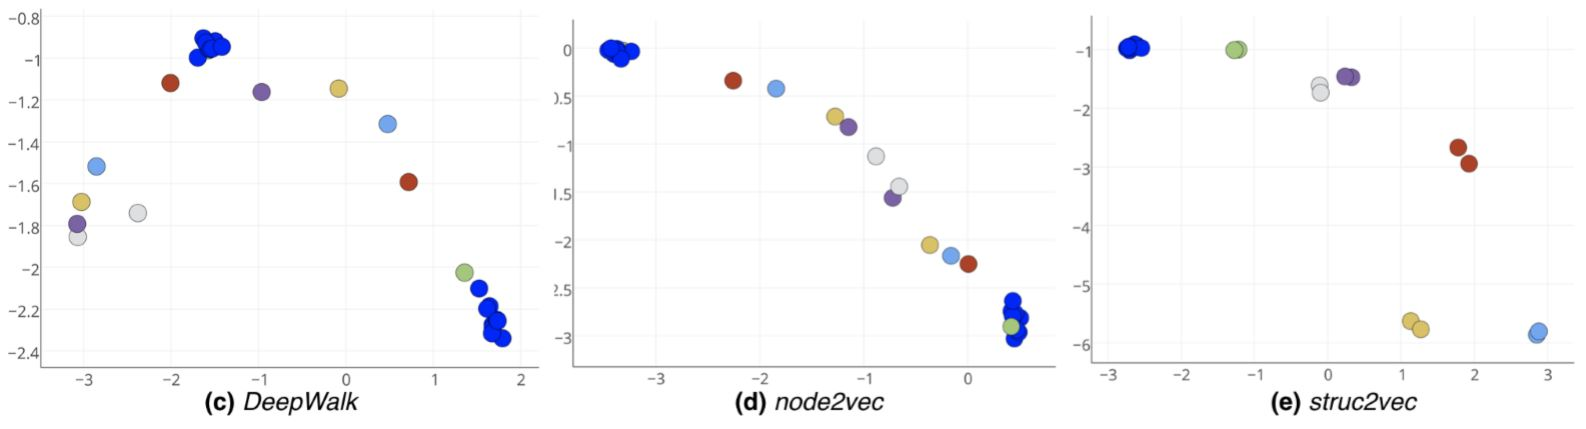
\includegraphics[scale=0.4]{struc2}

\begin{small}\textit{\textbf{Figura 9.3}: Confronto di struc2vec con due algoritmi allo stato dell'arte; il metodo eccelle nell'individuazione di structural identity fra nodi}.\end{small}
\end{center}

Un secondo test ha previsto l'utilizzo della \textit{Zachary's Karate Club network}, una rete composta da 34 nodi e 78 archi, nella quale ogni nodo rappresenta un membro del club e gli archi denotato un'interazione (esterna al club) fra due membri (informalmente, una relazione di "amicizia"). La rete è stata duplicata (si veda la \textit{\textbf{Figura 9.4}}) in due grafi $G_1$ e $G_2$ nei quali ogni nodo in $G_1$ possiede un corrispettivo \textit{specchio} in $G_2$. I due grafi sono stati connessi tramite un arco fra i nodi 1 e 37.
 
\begin{center}
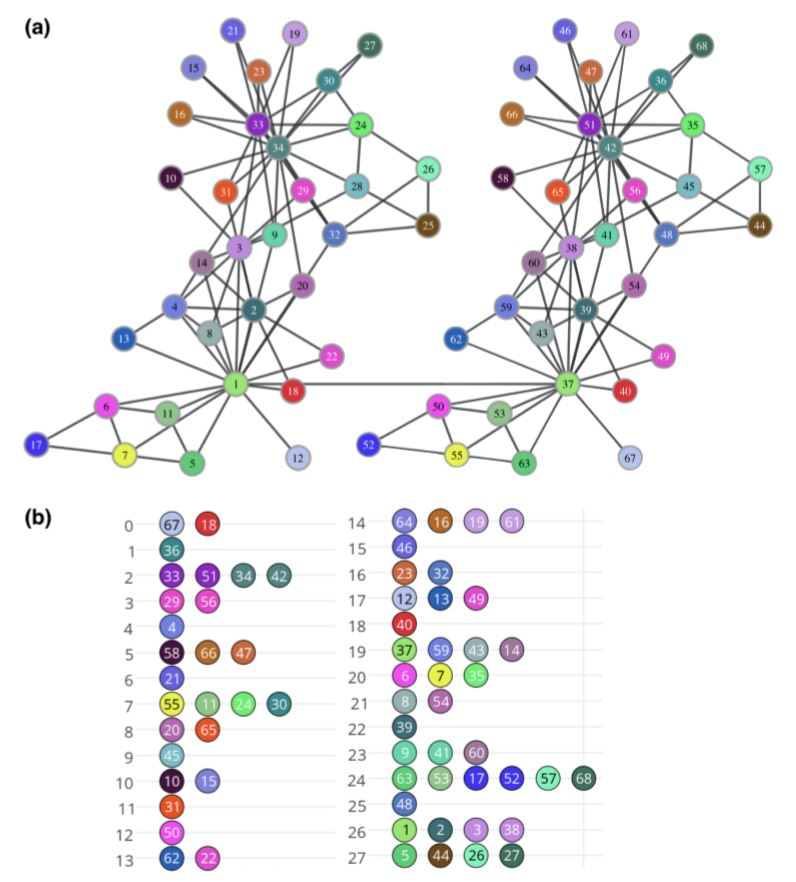
\includegraphics[scale=0.56]{struc4}

\begin{small}\textit{\textbf{Figura 9.4}: Zachary's Karate Club network con nodi specchio}.\end{small}
\end{center}

Anche in questo esempio \textit{DeepWalk} e \textit{node2vec} falliscono nell'individuare le \textit{latent representations} di nodi strutturalmente equivalenti (inclusi i nodi \textit{specchio}), mentre \textit{struc2vec} fornisce i risultati migliori.

\begin{center}
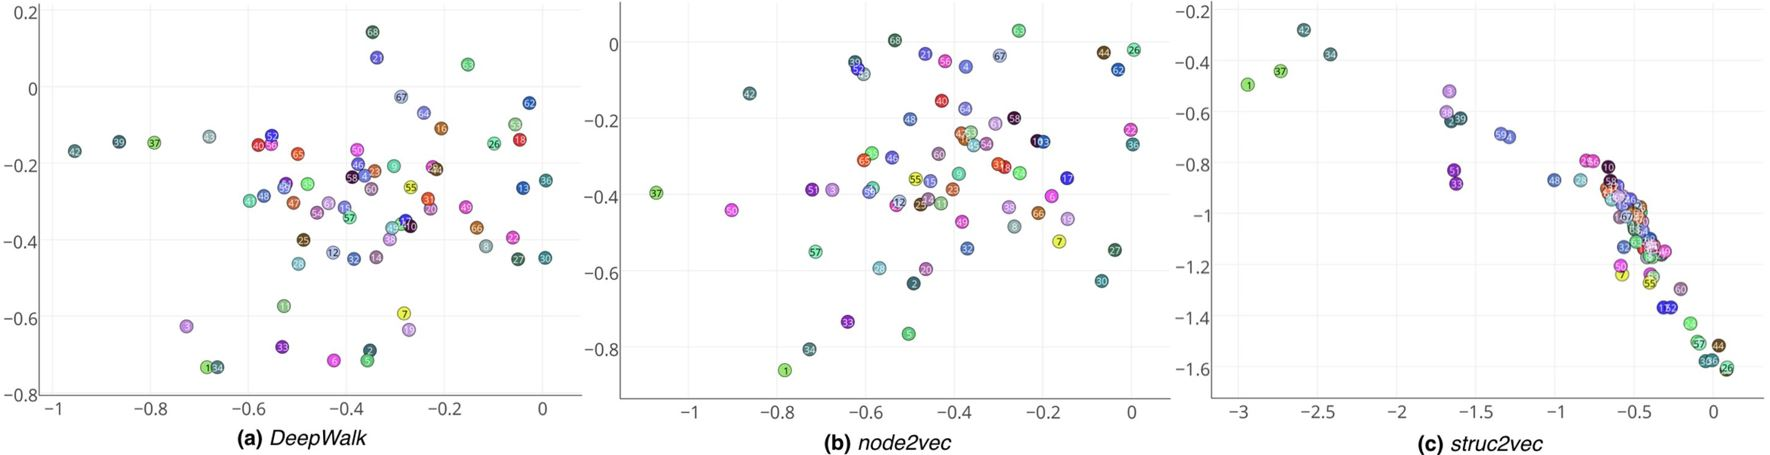
\includegraphics[scale=0.35]{a4}

\begin{small}\textit{\textbf{Figura 9.5}: Secondo test: confronto di struc2vec con i due algoritmi allo stato dell'arte}.\end{small}
\end{center}

Per concludere, ci teniamo a sottolineare il fatto che \textit{struc2vec} è stato citato 302 volte (fonte: Google Scholar) e per gli ambiti più differenti. \`E stato confrontato con un metodo sviluppato l'anno successivo, \textit{Deep Recursive Network Embedding} (DRNE), sullo stesso dataset; le prestazioni rimangono tutt'ora molto elevate.

\pagebreak
\section{L-GRAAL}
Sviluppato nel 2015, L-GRAAL -\textit{Lagrangian graphlet-based network aligner} - è un metodo basato sull'idea di mappare insieme nodi che costituiscono un pattern (presenza di sottografi chiamati \textit{graphlet}\footnote{I \textit{graphlet} sono sottografi di piccole dimensioni, connessi, non-isomorfici, indotti da un grafo più grande (sono indicati come G$_0$,...,G$_{29}$ nella \textit{\textbf{Figura 10.1}}).}) definito da una grande quantità di interazioni condivise. L-GRAAL ottimizza una funzione obiettivo, che fonde le informazioni derivanti dalle sequenze di proteine con le interazioni tra i vari \textit{graphlet}, risolta con la Programmazione Intera. L-GRAAL è in grado di individuare l'\textit{overlap} tra le reti e fornisce risultati migliori di tutti gli altri metodi GO-based a livello di \textit{mapping} delle proteine e delle interazioni tra le stesse.\\

Date due PPIN, $N_1 = (V_1, E_1)$ e $N_2 = (V_2, E_2)$ (con $|V_1| \leq |V_2|$, un \textit{allineamento globale}, $f: V_1 \rightarrow V_2$, è un mapping 1-a-1 dei nodi di $V_1$ con quelli di $V_2$. Ad un \textit{allineamento globale} viene associato uno score $S$:
\begin{center}
$S(f) = \displaystyle{\sum_{u \in V_1}n(u,f(u))} + \displaystyle{\sum_{(u,v) \in E_1}e(u,f(u),v,f(v))}$
\end{center}
dove $n : V_1 \times V_2 \rightarrow \mathbb{R}^+$ corrisponde allo score del mapping tra un nodo di $V_1$ e uno di $V_2$, mentre $e : E_1 \times E_2 \rightarrow \mathbb{R}^+$ corrisponde allo score del mapping tra un arco di $E_1$ e uno di $E_2$. Il \textit{Global Network Alignment problem} cerca di trovare un allineamento globale in grado di massimizzare $S$.

\subsection{\textit{Similarity scores} e funzione obiettivo}
In L-GRAAL si misura la relazione tra due proteine mappate $u$ e $f(u)$ utilizzando il loro allineamento di sequenza BLAST\footnote{BLAST è un algoritmo usato per comparare le informazioni contenute nelle strutture biologiche primarie.}:
\begin{center}
$n(u,f(u)) = \displaystyle{\frac{seqsim(u,f(u))}{max_{i,j}seqsim(i,j)}}$
\end{center}
dove $seqsim$ può essere un qualsiasi tipo di \textit{sequence-based similarity score}. Viene successivamente misurata la \textit{topological similarity} fra due proteine $u$ e $f(u)$ utilizzando il loro da 2- a 4-\textit{node graphlet degree similarity}\footnote{I \textit{graphlet} generalizzano il concetto di "grado di un nodo": il \textit{graphlet degree} di un nodo $v$, indicato con $d^i_v$ è il numero di volte che il nodo $v$ tocca un \textit{graphlet} all'orbita $i$. Vengono utilizzati per misurare la distanza tra due reti e le \textit{topological similarities} tra i nodi nelle reti.} $t$:
\begin{center}
$t(u,f(u)) = \frac{1}{15}\displaystyle{\sum \limits_{i=0}^{14}\frac{min(d_u^i,d_{f(u)}^i)}{max(d_u^i,d_{f(u)}^i}}$
\end{center}
Viene calcolata la \textit{topological similarity} fra due interazioni mappate (archi), $(u,v)$ e $(f(u),f(v))$, in base al loro \textit{graphlet degree similarity} dei loro nodi terminali mappati:

\begin{center}
$e(u,f(u),v,f(v)) = \displaystyle{\frac{1}{2}(t(u,f(u))+t(v,f(v)))}$
\end{center}
Lo score $e(u,f(u),v,f(v)) \in [0,1]$ e rewards mapping edges that are involved in similar local wiring patterns.

\begin{center}
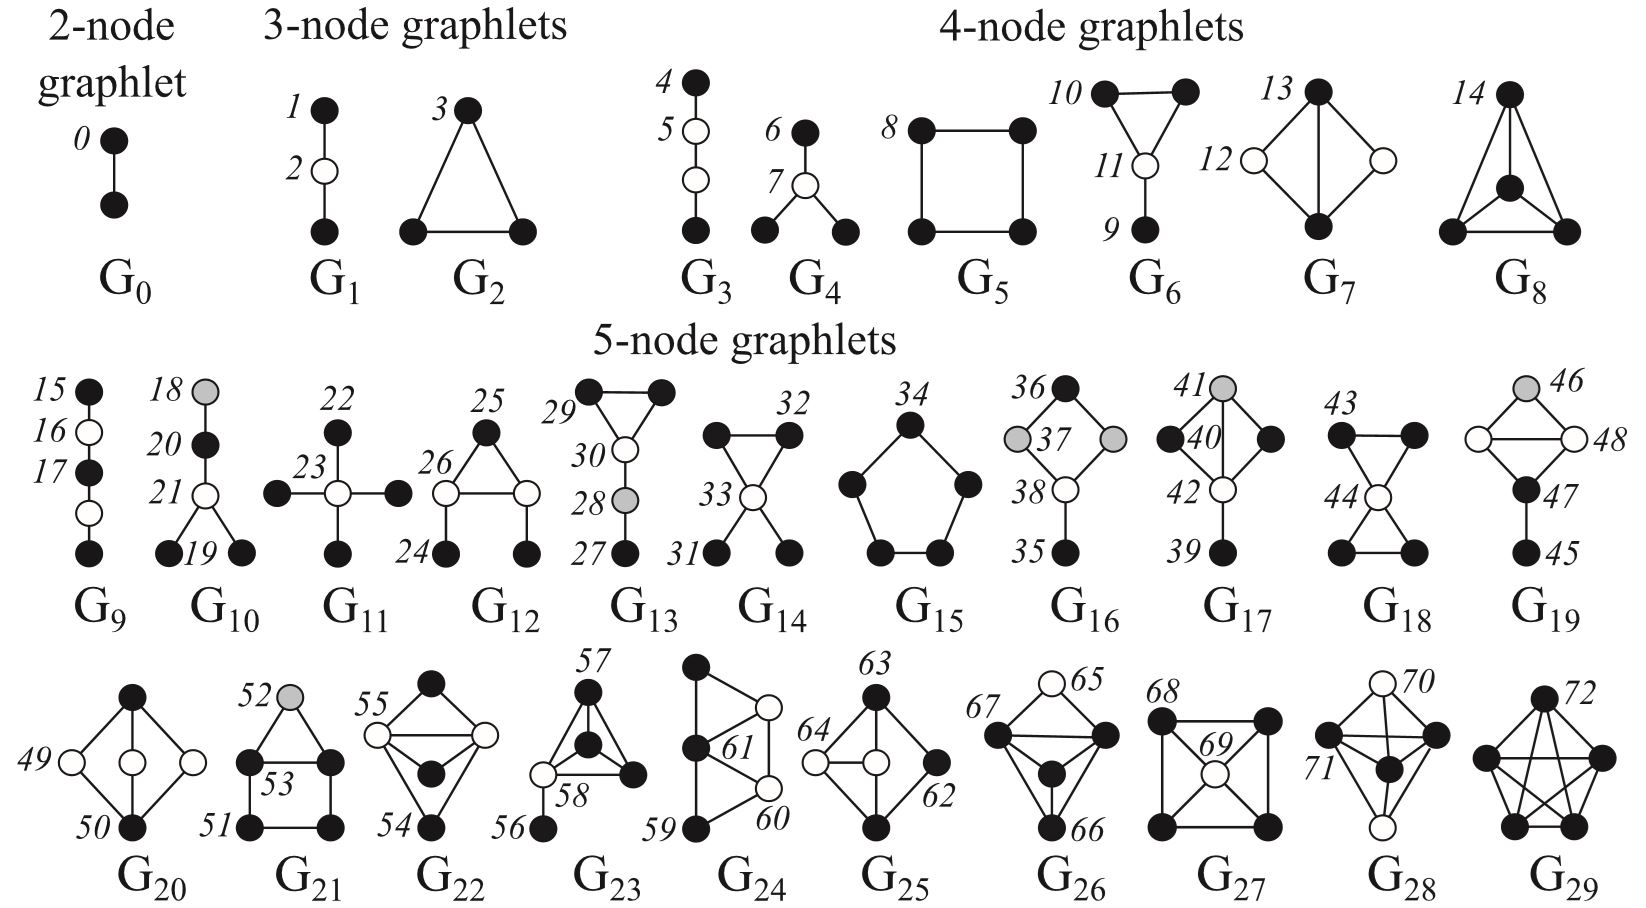
\includegraphics[scale=0.33]{graal1}

\begin{small}\textit{\textbf{Figura 10.1}: 2- to 5- graphlets e le loro automorphism orbits}.\end{small}
\end{center}

La funzione obiettivo di L-GRAAL, $S$, favorisce la relazione tra le proteine che vengono mappate o tra la \textit{topological similarity} tra le interazioni mappate, in accordo ad un parametro di \textit{balancing} $\alpha \in [0,1]$:
\begin{center}
$S(f) = \alpha \times \displaystyle{\sum_{u}n(u,f(u)) + (1- \alpha) \times \sum_{u,v}e(u,f(u),v,f(v))}$
\end{center}

\subsection{Strategia di ricerca \textit{two-step alignment}}
A causa della grande dimensione delle PPIN, risolvere il problema dell'allineamento delle reti cercando di considerare tutti i possibili mapping tra i nodi è, dal punto di vista computazionale, impossibile. L-GRAAL utilizza \textit{sequence} e \textit{graphlet degree similarities} per selezionare un sottoinsieme di nodi mappati $u \longleftrightarrow v$ di modo che $\alpha n(u,v) + (1-\alpha)t(u,v) \geq 0.5$. L'algoritmo applica successivamente un algoritmo \textit{greedy} per estendere la ricerca degli allineamenti. Il \textit{network alignment problem} può essere espresso tramite la seguente formula:

\begin{center}
IP $= max_{x,y} \displaystyle{\Big( \alpha \sum n(i,k) \times x_{ik} + (1- \alpha) \sum e(i,j,k,l) \times y_{ijkl}} \Big)$
\end{center}
soggetta ai vincoli:
\begin{center}
$\displaystyle{\sum_{k \in V_2}x_{ik} \leq 1}$, $\forall i \in V_1$,

$\displaystyle{\sum_{i \in V_1}x_{ik} \leq 1}$, $\forall k \in V_2$,

$x_{ij} - y_{ijkl} \geq 0$, $\forall (i,j) \in E_1, \forall (k,l) \in E_2$,

$x_{ik} - y_{ijkl} \geq 0$, $\forall (i,j) \in E_1, \forall (k,l) \in E_2$
\end{center}

dove, al \textit{node mapping} selezionato, $i \longleftrightarrow k$ con $i \in V_1$, $k \in V_2$, viene associata una variabile binaria $x_{ik} = 1$ se il \textit{node mapping} appartiene all'allineamento, 0 altrimenti. In modo del tutto simile, associamo ad ogni \textit{edge mapping} selezionato $(i,j) \longleftrightarrow (k,l)$, $(i,j) \in E_1$, $(k,l) \in E_2$, una variabile binaria $y_{ijkl} = 1$ se l'\textit{edge mapping} appartiene all'allineamento, 0 altrimenti. I primi due vincoli obbligano un nodo in $V_1$ ad essere mappato al massimo in un nodo di $V_2$ e viceversa, mentre gli ultimi due vincoli obbligano l'\textit{edge mapping} $(i,j) \longleftrightarrow (k,l)$ ad avere gli \textit{end-nodes} mappati: $i \longleftrightarrow k$ e $j \longleftrightarrow l$.

Si risolve l'equazione
\begin{center}
$LR(\lambda) = max_{x,y} \displaystyle{\sum n^{\lambda}(i,k) \times x_{ik} + \sum e^{\lambda}(i,j,k,l) \times y_{ijkl}}$
\end{center}

con la Programmazione Intera in $O(|V|^3 + |V|^2 \times d^3)$, dove $|V|$ è il numero di nodi nelle reti e $d$ è il valore del grado (di un nodo) massimo. Risolvere $LR(\lambda)$ genera una soluzione rilassata del problema, che corrisponde ad un \textit{upper bound} alla Programmazione Intera. 

Per risolvere tale problema nella sua interezza è necessario ricondursi alla formulazione duale per minimizzazare $LR(\lambda)$ su $\lambda)$ con la tecnica del \textit{gradient descent}. Sfortunatamente, anche questo problema è $\mathcal{NP}$-completo e, in pratica, si risolve generando una sequenza finita di interazioni. L'algoritmo restituisce il risultato dopo un determinato limite temporale o dopo un numero di iterazioni fissato.\\

Tutti i test, eseguiti su di un computer desktop con processore Intel Core i7-2600 a 3.40 GHz e una memoria RAM da 64 GB, hanno mostrato il grande potenziale di L-GRAAL (come mostrato dalla \textit{\textbf{Figura 10.2}}).

\begin{center}
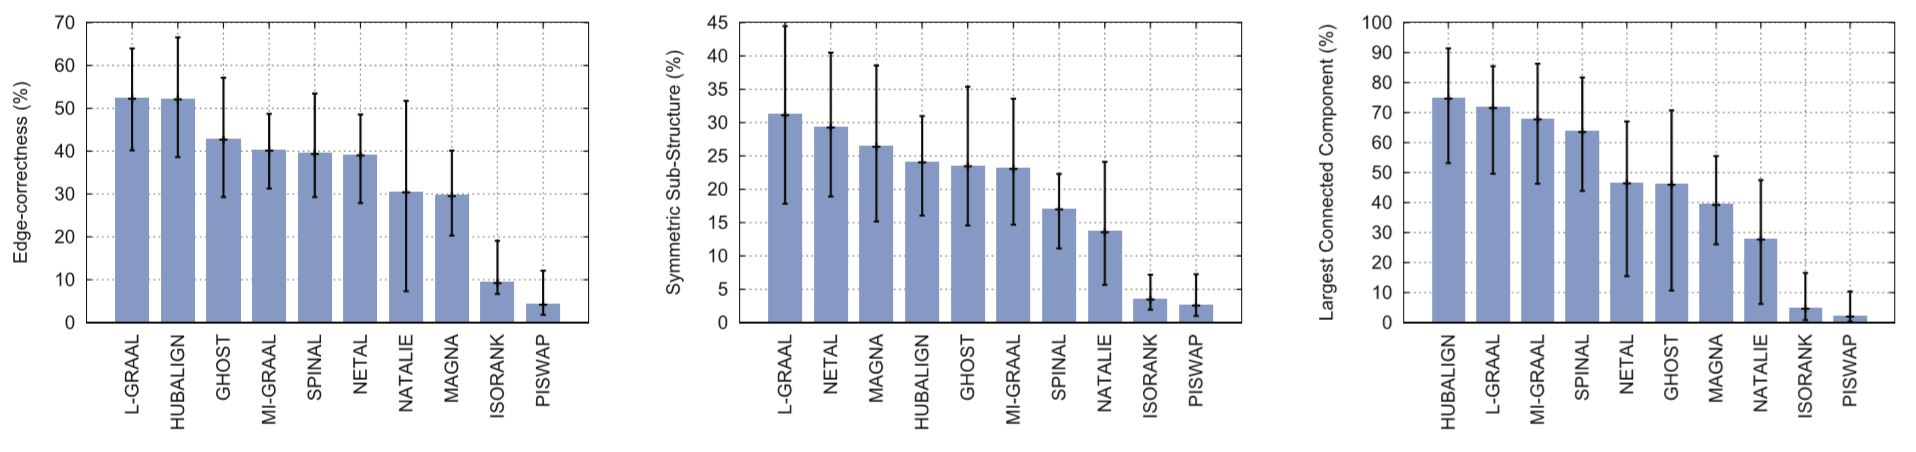
\includegraphics[scale=0.33]{graal2}

\begin{small}\textit{\textbf{Figura 10.2}: Confronto L-GRAAL vs altri metodi}.\end{small}
\end{center}

I metodi considerati sono stati inizialmente confrontati in base alla loro capacità di mappare le proteine che sono collegate in modo simile in entrambe le reti PPI. Nel primo grafico viene mostrata la percentuale di interazioni dalla rete più piccola mappate ad interazioni nell'altra rete. Poiché questa percentuale può essere ottenuta mappando regioni sparse della rete più piccola in regioni densamente connesse di quella più grande, misuriamo, contemporaneamente, anche quanto sono topologicamente simili  le regioni mappate usando \textit{symmetric sub-structure score}, che è la percentuale degli archi conservati tra la rete più piccola e la sottorete dalla rete più grande indotta dall'allineamento (si veda il secondo grafico). Infine, utilizziamo la dimensione del componente connesso più grande (\textit{largest connected component}, LCC) per garantire che gli allineamenti corrispondano ad una grande sottostruttura, comune, connessa, invece che a diverse piccole sottostrutture disconnesse.\\

In tutti i test svolti, il metodo L-GRAAL (citato 95 volte su Google Scholar negli ultimi anni 5 anni) ha mostrato una percentuale di successo non indifferente e uguale (a volte addirittura superiore) a tutti gli altri (si pensi ad esempio ad IsoRank, presentato nella \textit{\textbf{Sezione 8}}), in particolare con metodi testati per lo stesso problema e sullo stesso dataset.\\



\pagebreak
\section{Conclusioni}
Negli ultimi anni, il corpus di dati PPI è cresciuto esponenzialmente e il rapido ritmo di accumulo dati continua imperterrito tutt'oggi. L'obiettivo di questo progetto è stato di far capire la struttura delle reti di interazione proteina-proteina e le implicazioni dal punto di vista biologico.

Scoprire e capire i pattern all'interno delle PPIN è un problema centrale in Biologia. Gli allineamenti tra queste reti permettono di scoprire informazioni su complessi proteici che fino a pochi anni fa non erano note. 

Abbiamo proposto una descrizione, seppur breve, del funzionamento di quattro dei metodi più all'avanguardia proposti negli ultimi anni: MTGO, IsoRank, \textit{struc2vec} e L-GRAAL; metodi con un'elevata complessità dal punto di vista computazionale a causa dell'$\mathcal{NP}$-completezza del problema.\\

Molte sfide sono ancora aperte e molte frontiere devono ancora essere esplorate; con questo progetto abbiamo solamente dato una vaga idea della vastità dell'argomento, di cui si è appena iniziato a parlare.\\
\\
\\
\\
\\
\\
\\
\\
\\
\\
\begin{flushright}
\textit{Luca Masiero}\\
\textit{Stefano Ivancich}
\end{flushright}

\pagebreak 
\section{Bibliografia \& Sitografia} 
\begin{enumerate}
\item https://www.ebi.ac.uk/training/online/course/network-analysis-protein-interaction-data-introduction

\item https://www.ebi.ac.uk/training/online/course/goa-and-quickgo-quick-tour/what-go

\item Vella, D., Marini, S., Vitali, F. et al. MTGO: PPI Network Analysis Via Topological and Functional Module Identification. Sci Rep 8, 5499 (2018). https://doi.org/10.1038/s41598-018-23672-0

\item Mitra, K., Carvunis, A., Ramesh, S. et al. Integrative approaches for finding modular structure in biological networks. Nat Rev Genet 14, 719–732 (2013). https://doi.org/10.1038/nrg3552

\item No\"el Malod-Dognin, Nata\v{s}a Pr\v{z}uli. L-GRAAL: Lagrangian graphlet-based network aligner. Department of Computing, Imperial College London, London, UK (2015)

\item Ribeiro, Saverese, Figueiredo. \textit{struc2vec}: Learning Node Representations from Structural Identity. Federal University of Rio de Janeiro, Systems Eng. and Comp. Science Dep. (2017)

\item Singh, Xu, Berger. Global alignment of multiple protein interaction networks with application to functional orthology detection. Computer Science and Artificial Intelligence Laboratory and Department of Mathematics, Massachussets Institure of Technology, Cambridge, MA 02139; and Toyota Technological Institute at Chicago, Chicago, IL 60637 (2008)

\end{enumerate}
\end{document}
